\documentclass{article}
\usepackage[utf8]{inputenc}
\usepackage{amsfonts} 
\usepackage{amssymb}
\usepackage{amsmath}
\usepackage{mathtools}
\usepackage{mathalfa}
\usepackage{enumitem}
\usepackage{graphicx}
\usepackage[hidelinks]{hyperref}
\graphicspath{ {./images/} }

\title{Definizioni e Teoremi di Algebra (senza esempi)}
\author{Per comunicare errori o versioni aggiornate etc.:\\
  \href{https://github.com/Ianneee/Algebra\_Malvenuto\_definizioni}{https://github.com/Ianneee/Algebra\_Malvenuto\_definizioni}}
\date{Anno accademico 2021/2022}

\begin{document}

\maketitle

\tableofcontents
\section{Capitolo 1}
Relazione e corrispondenza sono interscambiabili.

\subsection{Corrispondenza}
Una corrispondenza \(\rho\) di X in Y è una terna ( \(\rho, X, Y\)) dove \(\rho \subseteq X\times Y\).

\subsection{Relazione in se}
Una Relazione di \(X\) in sè, è una corrispondenza \(\rho\) di X in X.
Se \((x, y) \in\rho\) si scrive anche \(x\rho y\)(notazione infissa), cioè x è in relazione \(\rho\) con y.

\subsection{Relazione/Corrispondenza inversa} 
Una corrispondenza \(\rho\) di X in Y è la relazione di Y in X denotata con \(\rho ^{-1}\) data dalla seguente:
\[y\rho^{-1}x \Leftrightarrow x\rho y\]

\subsection{Relazione di equivalenza} una relazione su A (cioè un sottoinsieme \(\rho\) di AxA) si dice di equivalenza se verifica le tre seguenti proprietà:

\textit{Riflessiva:} \(\forall a \in A, a\rho a\).

\textit{Simmetrica:} \(\forall a,b\) in \(A, a\rho b \Rightarrow b\rho a\)

\textit{Transitiva:} \(\forall a, b, c \in A\) se \((a\rho b \wedge b\rho c) \Rightarrow a\rho c\)

\subsection{Relazione banale (di uguaglianza)} 
Su A \(x, y \in A\) \(x\rho y \Leftrightarrow x=y\)

\subsection{Relazione caotica} 
Su A \(x\rho y\; \forall x,y \in A\)

\subsection{Classe di equivalenza} 
Data la relazione \(\rho\) in A, si definisce classe di equivalenza modulo \(\rho\) di un elemento \(a \in A\) l'insieme di tutti gli elementi che sono equivalenti ad \(a\); si denota con \([a]_\rho\).

\[[x]_\rho :=\{y\in A : y\rho x\} \]

\subsection{Insieme quoziente} 
Data la relazione di equivalenza \(\rho\) su A, si definisce insieme quoziente l'insieme delle classi di equivalenza di \(\rho\) dato \(x\in A\) si denota con \(A/_\rho\).
\[A/_\rho = \{[x]_\rho : x \in A \} \]
\newline
Nota: Relazione di equivalenza e partizioni insiemistiche sono sostanzialmente la stessa cosa.

\subsection{Partizione insiemistica} 
Una partizione insiemeistica di A è una famiglia di sottoinsiemi di A non vuoti, tali che ad ogni elemento di A corrisponde un solo sottoinsieme.
\[H = \{A_i : i \in I \} \] con \[A_i \subseteq A\; \forall i \in I\]
con
\[i \neq j,\;\; i,j \in I \Leftrightarrow A_i \cap A_j=\emptyset \]
che equivale a dire:
\[\cup_{i\in I} \; A_i = A\]
cioè la famiglia H ricopre A.

\subsection{Funzione/Applicazione} 
\(f:S\rightarrow T\) è un'applicazione di S in T se (f, S, T) è una corrispondenza di S in T, ovvero \(f\subseteq S\times T\) che soddisfa la seguente proprietà:
\\
\(\forall x \in S \; \exists !\) y in T denotato con \(y=f(x)\), f è una legge univoca (ben definita).
\\\\
L'elemento f(x) si chiama \textbf{immagine dell'elemento}.
\\\\
\textbf{L'immagine di f} è un sottoinsieme del codominio T definito da:
\[Im(f) := \{y \in T : \exists\; x \in S, y=f(x)\}\]
\newline
\textbf{Controimmagine di y} è il sottoinsieme di S del dominio definito da:
\[f^{-1}(y):=\{x\in S:f(x)=y\}\subseteq S\]

\subsection{Iniettiva} 
f è iniettiva \(\Leftrightarrow \forall x, x' \in S :[f(x)=f(x')\Rightarrow x=x']\).
\\\textit{Definizione alternativa:} f è iniettiva \(\Leftrightarrow \forall x,x' \in S : [f(x)\neq f(x') \Rightarrow x\neq x']\).
\\
f è iniettiva \(\Leftrightarrow \forall y \in T \; |f^{-1}|\leq 1\), ovvero per ogni elemento y in T esiste al più un'immagine.

\subsection{Suriettiva} 
f è suriettiva se \(\Rightarrow \forall y\in T \;\;\exists\; x \in S : f(x)=y\)
\\
\textit{Definizione alternativa:} f è suriettiva \(\Leftrightarrow f(S) = Im(S) = T\).
\\
f è suriettiva \(\Leftrightarrow \forall y \in T \; |f^{-1}(y)|\geq 1\), ovvero per ogni elemento y in T esiste almeno un'immagine.

\subsection{Biunivoca (biiettiva)} se f è sia iniettiva che suriettiva.
\\
f è biiettiva \(\Leftrightarrow \forall y \in T \; |f^{-1}(y)|=1\), ovvero per ogni elemento y in T esiste una sola immagine.

\subsection{Funzione caratteristica} 
E' la funzione che vale 1 se \(x \in S\), 0 se \(x \notin S\).

\subsection{Operazione binaria} 
Un'operazione binaria su S, è un'applicazione \(m:S\times S \rightarrow S\); notazione funzionale \((s, s') \mapsto m(s, s')\); notazione infissa \(sms'\) o \(s*s\).

\subsection{Assiomi di Peano} per la costruzione dei naturali \(\mathbb{N}\)
\begin{enumerate}
    \item I numeri formano una classe
    \item Lo "zero" è un numero
    \item Se \(a\) è un numero allora il successore \(a'\) è un numero
    \item Se \(a\neq b\) sono due numeri allora \(a'\neq b'\)
    \item Lo "zero" non è successore di nessun numero (\(\nexists \; a\) numero tale che \(zero=a'\))
    \item Assioma di induzione:
    \\Se S è una classe di numeri tale che:
    \begin{itemize}
        \item \(zero\in S\)
        \item Se \(a\in S\) allora \(a'\in S\)
    \end{itemize}
    allora ogni naturale è in S.
\end{enumerate}
I naturali sono la più piccola classe che 
\begin{itemize}
    \item Contiene lo zero
    \item Chiusa rispetto a contenere i successori
\end{itemize}

\subsection{Principio del buon ordinamento di \(\mathbb{N}\)} 
Se \(S\subseteq \mathbb{N}, S\neq\emptyset\), allora esiste un minimo in S, cioè esiste \(m\in S\) tale che se \(h\in\mathbb{N}, h<m\) allora \(h\notin S\).

\subsection{Teor: Divisione con resto su \(\mathbb{N}\)} 
Siano \(a,b\in\mathbb{N}, b\neq 0\); allora esistono \(q, r\in\mathbb{N}\) tali che
\begin{itemize}
    \item \(a=bq+r\)
    \item \(0\leq r<b\)
\end{itemize}
\(\forall a,b\in\mathbb{Z}, b\neq 0; \exists\) unici \(q, r\in\mathbb{Z}\) con \(a=bq+r \land 0\leq r<b\)
\\\textbf{Dimostrazione} per induzione:
\\\textit{Base:} $P(0),\; a=0$:
\\\\$\exists !q,r$ con $0=qb+r$ e $0\leq r <b$?
\\Prendo $q=0,\; r=0$ e si ha $0=0b+0,\;\;0\leq r=0<b$.
\\\\\textit{Ipotesi induttiva:} $\forall\; 0\leq k<a$ esistono quoziente e resto.
\\\\\textit{Passo induttivo:} due casi:
\begin{enumerate}
  
\item $a<b$:
  \[\Rightarrow a=b0+a,\; 0\leq a=r<b\]

\item $a\geq b\;\;(b>0)$
  \\Consideriamo $a-b=a'$:
  \[0\leq a-b<a\]
  \[0\leq a' <a\]
  $a'$ è uno dei $k$: $\forall k: \; 0\leq k<a$ vale $P(k)\Rightarrow P(a')$ cioè esistono $q', r'$ tali che:
  \[a'=bq'+r',\;\;0\leq r'<b\]
  \[\Rightarrow a=a'+b\Rightarrow a=q'b+r'+b=\]
  \[=(q'+1)b+r',\;\;0\leq r'<b\]
\end{enumerate}

\section{Calcolo combinatorio}

\subsection{Notazione funzionale} 
Insieme delle applicazioni da A verso B
\[B^A=\{f:A\rightarrow B\}\]

\subsection{Fattoriale crescente} 
\[n^{(m)}:= n\ast (n+1)\ast ... \ast (n+m-1)\]

\subsection{Fattoriale decrescente} 
\[n_{(m)}:= n\ast (n-1)\ast ... \ast (n-m+1)\]

\subsection{Pigenhole principle (principio dei cassetti)} 
Se ho \textit{n} oggetti e \textit{m} cassetti, se \(n>m\) e devo disporre tutti gli oggetti nei cassetti allora esiste un cassetto che contiene almeno due oggetti.

\subsection{Permutazione} 
Sia A un insieme. Una biiezione \(f:A\rightarrow A\) si chiama anche \textit{permutazione} di A.

\subsection{Coefficiente binomiale}
\textbf{Prima interpretazione combinatoria:} \(\binom{n}{i}\) è il coefficiente di \(x^i y^{n-i}\) nello sviluppo \((x+y)^n=\sum _{z_i\in \{x,y\}} z_1 ...z_n\), ovvero il numero di stringhe binarie (su {x, y})
\begin{itemize}
    \item lunghe n
    \item con i occorrenze di x
    \item con n-i occorrenze di y
    \item \((x+y)^n =\sum _{i=0} ^n\binom{n}{i} x^iy^{n-i}\)
\end{itemize}
\noindent\textbf{Seconda interpretazione combinatoria:} numero di sottoinsiemi di cardinalità \textit{i} su un insieme \([n]\) di cardinalità \textit{n}.

\subsection{Formula} 
\[\binom{n}{i}=\frac{n(n-1)\ast ... \ast (n-i+1)}{i!} = \frac{n!}{i!(n-i)!}\]

\subsection{Relazione ricorsiva}
\[\binom{n}{i}=\binom{n-1}{i-1}+\binom{n-1}{i}\]
Dimostrazioni algebrica e combinatoria.

\subsection{Simmetria}
\[\binom{n}{i}=\binom{n}{n-i}\]
Il coefficiente binomiale è simmetrico rispetto al centro della riga n-esima \(\lfloor\frac{n}{2}\rfloor\) del triangolo rappresentante tutti i coefficienti del coefficiente binomiale.

Dimostrazioni algebrica e combinatoria.

\subsection{Relazione d'ordine}
Una relazione \(\rho\) su \textit{X} è una relazione d'ordine (o un ordine, o un ordinamento) se valgono per \(\rho\) le proprietà:
\begin{itemize}
    \item (R) \(\forall x, x\rho x\)
    \item (AS) \(\forall x,y\; (x\rho y\land y\rho x)\Rightarrow x=y\)
    \item (T) \(\forall x,y,z\; (x\rho y\land y\rho z)\Rightarrow x\rho z\)
\end{itemize}

\subsection{Proposizione - Naturali e divisibilità}
$(\mathbb{N}, |)$ l'insieme dei naturali con la divisibilità è un insieme parzialmente ordinato. (La divisibilità è una relazione d'ordine su $N*$).
\\TODO: Dimostrazione R, AS, T

\subsection{POSET (Partial order set)}
Un insieme munito di una relazione d'ordine si dice parzialmente ordinato.

\section{I numeri}
\subsection{Costruzione di \(\mathbb{Z}\) (interi)} 
Partendo da \(\mathbb{N}\): prendiamo su \(\mathbb{N}\times\mathbb{N}\) la relazione \(\rho\) definita sulle coppie \((n, m)\in \mathbb{N}\times\mathbb{N}\) tale che \((n, m)\rho (n',m') \Leftrightarrow n+m'=m+n'\)

\subsection{Definizione di \(\mathbb{Z}\)} 
\[\mathbb{Z}=\mathbb{N}\times\mathbb{N}/_{\rho}\]

\subsection{Classi su \(\mathbb{Z}\)} 
\(\overline{(0,0)}\) zero
\\\(\overline{(m, 0)}, m>0\) positivi
\\\(\overline{(0, n)}, n>0\) negativi

\subsection{Sottoinsiemi di \(\mathbb{Z}\)} 
\[\mathbb{Z}=\mathbb{Z}^{>0}\cup\{0,0\}\cup\mathbb{Z}^{<0}\]

\subsection{Somma su \(\mathbb{Z}\)}
\[\overline{(n,m)}+\overline{(n',m')}=\overline{(n+n',m+m')}\]

\subsection{Prodotto su \(\mathbb{Z}\):}
\[\overline{(n,m)}\cdot\overline{n',m'}=\overline{(nn'+mm', nm'+mn')}\]

\subsection{Proprietà operazioni su \(\mathbb{Z}\)} 
\(\forall a,b,c\in\mathbb{Z}\) (\(a,b,c\) coppie \(\overline{(n,m)}\)) valgono le seguenti:
\begin{enumerate}
    \item Associatività: \((a+b)+c=a+(b+c)\)
    \item Commutatività: \(a+b=b+a\)
    \item Esiste uno \textit{zero} per la somma, cioè un elemento \(0: a+0=0+a=a\)
    \item \(\forall a\in\mathbb{Z}\) esiste un elemento detto \textit{opposto}, denotato con \(-a\), cioè un elemento tale che: \(a+(-a)=(-a)+a=0\).
    
    \(a=\overline{(n,m)}\)
    
    \(-a=\overline{(m,n)}\)
    \item Associatività prodotto: \(a\cdot (b\cdot c)=(a\cdot b)\cdot c\)
    \item Commutatività prodotto: \(a\cdot b=b\cdot a\)
    \item Esiste un \textit{elemento neutro} per il prodotto, "1", cioè un numero in \(\mathbb{Z}\) tale che:
    \[a\cdot 1=1\cdot a=a\]
    \[\overline{(n,m)}\cdot\overline{(1,0)}=\overline{(n,m)}\]
    \item Distributività del prodotto sulla somma:
    \[a\cdot (b+c)=a\cdot b+a\cdot c\]
\end{enumerate}

% Spostato in strutture algebriche
% \subsection{Gruppo} 
% Un insieme S non vuoto, munito di una operazione \[m:S\times S\rightarrow S\]
% \[(a,b)\mapsto m(a,b)=a\ast b\;\; (notazione\; infissa)\]
% che verifica i punti 1, 3, 4 si chiama \(gruppo(S,\ast)\).
% \\L'operazione su S è dunque:
% \begin{itemize}
%     \item associativa
%     \item con elemento neutro \textit{e}: \(\forall x, x\ast e=e\ast x=x\)
%     \item per ogni elemento \textit{x} esiste un inverso rispetto al prodotto \(\ast\) cioè un elemento \textit{y} tale che \(x\ast y=y\ast x=e\), che si denota \(x^{-1}\)
% \end{itemize}

% \subsection{Gruppo commutativo (abeliano)} 
% Se il gruppo \((S, \ast)\) soddisfa anche la proprietà 2 (quindi associatività,  elemento neutro, opposto, +commutatività).

% \subsection{Anello} 
% Un anello è una terna \((A,+,\cdot)\) con:
% \begin{itemize}
%     \item A insieme non vuoto
%     \item \(+ \; \cdot\) due operazioni binarie, associative
%     \item \((A,+)\) è un gruppo abeliano
%     \item Distributività: \(\forall a, b, c \in A, \; a\cdot (b+c)=a\cdot b+a\cdot c\)
% \end{itemize}

% \subsection{Anello commutativo} 
% Se un anello \((A,+,\cdot)\) il prodotto è commutativo, cioè se \(\forall a,b\in A,\;a\cdot b=b\cdot a\).

% \subsection{Anello unitario} 
% Se esiste un elemento di A, che si denota con \(1_A\), tale che \(a\cdot 1_A=1_A\cdot a=a\).

% \subsection{Divisore dello zero} 
% Un elemento \(a\in A,\; a\neq0_A\) di un anello di dice divisore dello zero se esiste \(b\in A,b\neq 0\) con \(a\cdot b=0_A\).

% \subsection{Dominio di integrità} 
% Se \((A,+,\cdot)\) è privo di divisori dello zero.

% \subsection{Legge di annullamento del prodotto} 
% Se in un dominio di integrità \(a\cdot b=0_A\) allora \(a=0_A\) oppure \(b=0_A\).

\subsection{Divisibilità} 
Dati \(a,b\in\mathbb{Z}\) si dice che a divide b, e si indica \(a|b\), se e solo se \(\exists c\in\mathbb{Z}\) tale che \(b=a\cdot c\) (ovvero \(a|b\Leftrightarrow\exists c\in\mathbb{Z}: b=a\cdot c\)).
\\La divisibilità è una relazione sugli interi:

\subsection{Multiplo} 
Se \(a|b\) diremo che \textit{b} è un multiplo di \textit{a}.

\subsection{Associati}
\textit{a,b} sono associate se \(a|b\) e \(b|a\)
\newline\textit{Oss1:} in \(\mathbb{N^*}\) sono associati \(\Leftrightarrow a=b\).
\newline\textit{Oss2:} in generale, in \(\mathbb{Z}\Leftrightarrow a=b\) oppure \(a=-b\).

\subsection{Unità}
In \(\mathbb{Z}\) sono +1 e -1.

\subsection{Irriducibile}
Un elemento \(a\in\mathbb{Z}, \; a\neq 0\) è irriducibile se \(a=b\cdot c\Rightarrow\) \textit{b} oppure \textit{c} sono unità.

\subsection{Primo}
Un elemento \(a\in\mathbb{Z}\) si dice primo se:
\[a|b\cdot c\Rightarrow a|b \;oppure\; a|c\]

\subsubsection{Proposizione: in \(\mathbb{Z},\; a\) è primo \(\Rightarrow\;a\) irriducibile}
Sia \(a=b\cdot c\): usando l'ipotesi che a è primo allora \(a|b\) oppure \(a|c\).
\\
Se \(a|b \Rightarrow\exists\; h : b=a\cdot h \Rightarrow a = a\cdot h\cdot c \Rightarrow h\cdot c=1\Rightarrow c=\pm 1\)
\\
Allora \(a=b\cdot (+1)\) oppure \(a=b\cdot (-1)\), \textit{a} è irriducibile.

\subsubsection{Proposizione: in \(\mathbb{Z}\) a irriducibile\(\Rightarrow\)a primo}
Ipotesi: \(a\) irriducibile
\\
Tesi: \(a\) primo
Supponiamo che \(a|bc\Leftrightarrow\exists h\in\mathbb{Z}:bc=ah\),
\\
voglio mostrare che \(a|b\) oppure \(a|c\) ovvero che se \(a\nmid b\) allora \(a|c\).
\\
Ora \(a\) irriducibile, i suoi divisori sono \(a,-a,1,-1\). \(a\nmid b\) allora anche \(-a\nmid b\Rightarrow\)i divisori comuni tra \textit{a} e \textit{b} sono \(1,-1\rightarrow MCD(a,b)=1\).
\\\\
\centerline{\(\exists\)(id. Bézout)\(\exists\; h,k\in\mathbb{Z}\)}
\[1=ah+bk\]
moltiplicando per \(c\)
\[c=cah+cbk=a(ck+k)\;\;\;[cb=a]\]
quindi \(a|c\).

\subsection{Massimo comune divisore}
Dati \textit{a,b} non entrambi nulli, un elemento \(d\in\mathbb{Z}\) si chiama massimo comune divisore tra \textit{a} e \textit{b} un numero tale che:
\begin{itemize}
    \item \(d|a \land d|b\)
    \item Se \(c|a \land c|b\), allora \(c|d\): \textit{d} è il massimo tra i divisori comuni.
\end{itemize}
Chiamiamo massimo comune divisore l'unico positivo che soddisfa le due proprietà.

\subsubsection{Teor: Esistenza del MCD tra due numeri}
\(\forall a,b\in\mathbb{Z}\) non entrambi nulli, esiste un numero \(d\in\mathbb{N^*}\) tale che \(d=MCD(a,b)\)
\\
Il massimo comune divisore si esprime come una combinazione lineare tra \textit{a} e \textit{b}, ovvero esistono \(s, t\in\mathbb{Z}\) tali che \(d=s\cdot a+t\cdot b\) (\textit{identità di Bézout}).

\textbf{Dimostrazione}:
\\
Sia \(S=\{xa+yb:x,y\in\mathbb{Z}, xa+yb>0\}\)
\begin{enumerate}
    \item \(S\subseteq\mathbb{N}\)
    \item \(S\neq\emptyset\)
\end{enumerate}
a e b sono non entrambi nulli, quindi almeno uno dei due è \(\neq 0\).
Sia esso a.
\\
Se \(a>0\) allora \(1\cdot a+0\cdot b=a>0\)
\\Se \(a<0\) allora \((-1)\cdot a+0\cdot b=a>0\)

Per il principio del buon ordinamento, $S$ ammette un elemento minimo: sia esso $d$.
Quindi ogni altra combinazione lineare che sia $<d$ non appartiene ad $S$.
\\\textbf{Dimostrazione che \(d|a\) e \(d|b\):}
\\
Dividiamo \textit{a} per \textit{d} (divisione col resto):
\(\exists\; q,r\) con \(a=dq+r,\; 0\leq r<d\)
\\
Se \(r=0\) allora \(d|a\)
\\
Se \(r\neq 0\) allora \(0<r<d\)
\\
\(r=a-dq\); dato che \(d\in S\Rightarrow d=x_0a+y_0b\) allora
\\ \(r=a-q(x_0a+y_0b)=a-qx_0a-qy_0b=a(1-qx_0)+(-qy_0)b\)
\\
Quindi \(r\in S\) perchè è una combinazione lineare \(>0\) ma \(r<d\), però \textit{d} è il minimo di \(S\Rightarrow\)Assurdo.
\\\\
Dimostrazione se \(d'|a\) e \(d'|b\) allora \(d'|d\):
\\
Poichè \(d'|a\) e \(d'|b\) si ha che
\[\exists h:a=d'\cdot h, \exists k:b=d'\cdot k\]
Ora \[d=x_0a+y_0b\]
\[=x_0(d'h)+y_0(d'k)=\]
\[=d'(x_0h+y_0h)\Rightarrow d'|d\]

\subsubsection{Prop: se \(c|a\) e \(c|b\) allora \textit{c} divide ogni combinazione lineare di a e b}
\[a=ch\]
\[b=ck\]
\[\Rightarrow xa+yb=xch+yck\]
\[=c(xh+yk)\Rightarrow\in\mathbb{Z}\]
\[\Rightarrow c|xa+yb\]

\subsection{Proposizione}
\[1=at+bs\Rightarrow MCD(a,b)=1\]

\subsubsection{Lemma MCD(m,m+1)=1}
Sia \(m\in\mathbb{N},\; m\geq 1\) allora \(MCD(m,m+1)=1\).
\\\\
\textbf{Dimostrazione}: \[m+1-m=1\Rightarrow 1(m+1)+(-1)m=1\]
Potendo scrivere \textit{1} come combinazione lineare di \textit{m} e \textit{m+1}, \textit{m} e \textit{m+1} sono primi tra loro.

\subsection{Algoritmo di Euclide}

\subsubsection{Lemma1: L'algoritmo termina}

La successione dei resti è un numero \(0\leq ... <r_2<r_1<b\).

\subsubsection{Lemma2: Se \(a=bq+r\) \(MCD(a,b)=MCD(b,r)\)}
Ogni divisore comune di $a$ e $b$ è anche divisore comune di $b$ ed $r$: questo dimostra che il $MCD(a,b)|MCD(b,r)$:
\\Sia $d\in\mathbb{N}$: $d|a\land d|b$ e ricavando $r$ da $a=bq+r$, si ha:
\[a=dh\;\;\;b=dk\]
\[r=a+b(-q)=dh+dk(-q)=d(h+k(-q))\]
$d|r$ perchè $r$ è combinazione lineare di $a$ e $b$.
\\In particolare il
\[MCD(a,b)|a\]
\[MCD(a,b)|b\]
si ha che il $MCD(a,b)|r$ e $MCD(a,b)|b$.
\\$\Rightarrow MCD(a,b)|MCD(r,b)$

\subsubsection{Corollario: \(MCD(a,b)=MCD(r_n,0)=r_n1\)}
Per il lemma 2 \(MCD(a,b)=MCD(b,r_1)=MCD(r_1,r_2)=...=MCD(r_{n-1},r_n)=MCD(r_n,0)\)

\subsubsection{Lemma3}
Se \(x\in\mathbb{N^*}\) allora \(MCD(x,0)=x\)

\subsection{Coprimi}
\textit{a,b} non entrambi nulli, \textit{a} e \textit{b} si dicono coprimi (o \textit{primi fra loro}) se \textit{MCD(a,b)=1}.

\subsubsection{Osservazione1}
Se \textit{a} e \textit{b} sono primi fra loro, allora \[\exists\; x,y\in\mathbb{Z} : 1=xa+yb\]

\subsubsection{Osservazione 2}
Se \[d=MCD(a,b)\Rightarrow\exists\; x,y:d=ax+by\]

\subsubsection{Proposizione 1}
Se \(\exists\; x_0,y_0\) con \(1=ax_0+by_0\) allora \textit{a,b} sono primi tra loro.

\subsubsection{Proposizione 2}
Se \textit{a} e \textit{b} sono coprimi e dividono un terzo numero \textit{c}, allora \(ab|c\).

\subsection{Equazione diofantea}
Equazione con una o più incognite sugli interi di cui si cercano le soluzioni intere. Sono del tipo:
\[ax+by=c\]

\subsubsection{Teor: Soluzione equazione diofantea}
L'equazione diofantea lineare in \textit{x} e \textit{y} \(ax+by=c\;\; a,b,c\in\mathbb{Z}\) possiede soluzioni intere \((x,y)\in\mathbb{Z}^2\Leftrightarrow d=MCD(a,b)|c\)
\\
(Dim\(\Rightarrow\)) La condizione \(MCD(a,b)|c\) è necessaria.
\\
Ipotesi: esiste una soluzione di \(x^2+y^2=z^2\)
\\
Tesi: \(d|\)termine noto, \(d=MCD(a,b): d|a\) e \(d|b\Rightarrow d|\) ogni combinazione lineare di \textit{a,b}.
\\
Se \(x_0,y_0\) sono una soluzione, allora \(ax_0+by_0=c\Rightarrow d|c=ax_0+by_0\)
\\\\
(Dim\(\Leftarrow\)) La condizione è sufficiente.
\\
Ipotesi \(MCD(a,b)=ah+bk\), per opportuni \(h,k\in\mathbb{Z}\)

\subsection{Teorema fondamentale dell'aritmetica}
\(\forall n>1, n\in\mathbb{N},\exists\;p_1,...,p_j\in\mathbb{N}\) (irriducibili) \(\exists h_1,...,h_j\geq 1\) tali che:
\begin{itemize}
    \item \(n=p_1^{h_1}...p_j^{h_j}\;\;p_1,...p_j\) distinti
    \item la fattorizzazione di \(n=p_1^{h_1}...p_j^{h_j}\;\;p_1,...p_j\) è unica a meno di riordinare i fattori
\end{itemize}

\subsubsection{Osservazione 1}
j può essere 1, cioè potrebbe esserci un solo irriducibile nella fattorizzazione di \textit{n}, anche \textit{h} possono essere 1.
Se \textit{n} è irriducibile \(\Rightarrow n=n\) è la fattorizzazione in irriducibili di \textit{n}.

\subsubsection{Osservazione 2}
1 non è considerato irriducibile perché si perderebbe l'unicità della scrittura in irriducibili.

\subsubsection{Dimostrazione esistenza}
Con principio di induzione in forma forte.
\\
\textbf{Base}: \textit{n=2}, 2 è irriducibile.
\\
Per \textbf{oss1} \(2=2^1\) è la fattorizzazione in primi in irriducibili di 2
\\
\textbf{Ipotesi induttiva}: ogni \(2\leq a<n\;\;(2\leq a\leq n-1)\) è fattorizzabile in irriducibili: \(\exists\; \alpha _1...\alpha _t \alpha _i\geq 1\) e \(q_1,...q_t\) irriducibili con \(a=q^{\alpha _1}_1...q_t^{\alpha _t}\)
\\
\textbf{Passo induttivo}: provare che \textit{n} sia prodotto di irriducibili
\\\\
\textbf{Primo caso}: \textit{n} irriducibile \(\rightarrow\) fatto, per \textit{oss.1}
\\\\
\textbf{Secondo caso}: \textit{n} riducibile: \(\exists\;b,c\in\mathbb{Z}, 1\neq b, c\neq n\) (divisori propri) con \(n=bc\Rightarrow 2\leq b,c<n\).
\\
Allora per \textit{b} e \textit{c} vale l'ipotesi induttiva e quindi
\[b=q_1^{\alpha _1}...q_t^{\alpha _t}\;\; c= x_1^{\beta _1}...x_s^{\beta _s}\]
\[n=bc=q_1^{\alpha _1}...q_t^{\alpha _t} x_1^{\beta _1}...x_s^{\beta _s}\]

\subsection{Dimostrazione unicità}
\textbf{Nota: le fattorizzazioni hanno gli esponenti}
\\Per induzione su \textit{m}, con \textit{m} è la lunghezza minima di una fattorizzazione per \textit{n}.
\\
\textit{m}: minimo numero di irriducibili di una fattorizzazione di \textit{n}
\\
\textbf{Base}: \(m=1\Rightarrow n=n\) è primo.
\\
Se per assurdo \(n=q_1...q_s,\; s\geq 2\) allora \(n|q_1\) o \(n|q_2...q_s\).
\\
Prendiamo \(n|q_1\), anche \(q_1\) è primo \(\Rightarrow n=q_1\); semplificando da entrambe le parti \(\Rightarrow 1=q_2....q_s\) che porterebbe ad un assurdo perché \(1=1\).
\\
Quindi \(n=q_1\) ed è l'unica fattorizzazione.
\\\\
\textbf{Ipotesi induttiva}: se il minimo numero di primi in una fattorizzazione di \textit{n} è \(m-1\), allora la fattorizzazione è unica a meno dell'ordine.
\\\\
\textbf{Passo induttivo}: Prendo $n$ con una fattorizzazione lunga $m$ irriducibili ed un altra fattorizzazione di $n$:
\[n=p_1p_2...p_m=q_1q_2....q_k\]
Prendo un $p_i$ che essendo primo dividerà uno dei $q_i$ e quindi usando la cancellatività a destra e sinistra, la fattorizzazione $p_1...p_{i-1}p_{i+1}...p_{m}$ sarà lunga $m-1$ irriducibili, allora per l'ipotesi induttiva la fattorizzazione lunga $m-1$ è unica $\Rightarrow$ anche la fattorizzazione di $n$ è unica.


\subsection{Teor. Euclide - Esistenza infiniti primi}
L'insieme \(P=\{p\in\mathbb{N} :\) p è primo\(\}\) è infinito.
\\
\textbf{Dimostrazione}: Supponiamo che \textit{P} sia finito, cioè \(P=\{p_1,...,p_n\}\).
\\
Sia \(m=p_1,...p_n\) il prodotto di tutti i primi.
\\
Considero \(m+1\): per il teorema fondamentale dell'aritmetica \(m+1=p_1^{k_1}...p_n^{k_n}\), \(k_1,...,k_n\geq 0\) almeno uno degli esponenti \(>0\).
\\
Per il lemma su MCD di un numero ed il suo successivo \textit{m} e \textit{m+1} sono coprimi.
\\
Sia \textit{j} tale che \(k_j>0\), cioè \(p_j^{k_j}|m+1\); vale anche \(p_j|m\) allora \(p_j|MCD(m, m+1)=1\) che è un assurdo.

\section{Congruenze}

\subsection{Congruenza modulo n}
La congruenza modulo n (n fissato) è una relazione di equivalenza definita su \(\mathbb{Z}\).

\(x\equiv y(mod\; n)\Leftrightarrow x-y\) multiplo di \textit{n} \(\Leftrightarrow n|x-y\)

\subsection{Proposizione}
La congruenza \textit{(mod n)} è una relazione di equivalenza.
\\
\textbf{Dimostrazione}:
\\\\
\textit{(R)} \[\forall x\in\mathbb{Z}: x\equiv x(mod\; n)\Leftrightarrow n|(x-x)\]
Vera perché \(0=0\cdot n\).
\\\\
\textit{(S)}
\[\forall x,y\in\mathbb{Z}: x\equiv y(mod\; n)\Rightarrow y\equiv x(mod\; n)\]
So che \(n|x-y\Leftrightarrow x-y=nh\) per qualche \(h\in\mathbb{Z}\).
\\\\
Moltiplicando per \textit{-1}: \(y-x=-nh=n(-h)\) quindi \(n|y-x\Rightarrow y\equiv x(mod\;n)\)
\\\\
\textit{(T)}
\[x\equiv y(mod\;n)\land y\equiv z(mod\;n)\Rightarrow x\equiv z(mod\;n)\]
\((x-y)=nh_1 \land (y-z)=nh_2\)
\\
\((x-z)=(x-y)-(y-z)=nh_1-nh_2=n(h_1-h_2)\) quindi \(n|x-z\Rightarrow x\equiv z(mod\;n)\)

\subsection{Quoziente}
Il quoziente della congruenza \textit{(mod n)} si denota come \(\mathbb{Z}_{/ \equiv (mod\;n)}=\{[x]_n:x\in\mathbb{Z}\}\).
\\
Il quoziente \(\mathbb{Z}_n\) si chiama anche \textbf{interi modulo n}.

\subsection{Proposizione - Resto}
Dati \(x,y\in\mathbb{Z}\) si ha: \(x\equiv y(mod\;n)\Leftrightarrow\) il resto delle divisioni di \textit{x} e di \textit{y} per \textit{n} è lo stesso.
\\
\textbf{Dimostrazione \(\Rightarrow\)(se \(x\equiv _n y\) hanno lo stesso resto}
\(x-y=nh\) (per qualche h)\\
\(x=nh+y\)\\
Dividendo \textit{y} per \textit{n}: \(\exists !q,r\in\mathbb{Z} : y=nq+r,\; 0\leq r<n\).
\\
Scambiando in \textit{x}: \(x=nh+nq+r=n(h+q)+r\), \textit{x} ed \textit{y} hanno quindi lo stesso resto.

\subsection{Osservazione}
Sia \(x=nq+r,\;0\leq r<n\) la divisione con resto di \textit{x} per \textit{n}.\\
Allora \[[x]_n=[r]_n\Leftrightarrow x\equiv r(mod\;n)\Leftrightarrow x-r=nq\]
Quindi \[n|x-r\]

\subsection{Proposizione somma}
La somma classi resto in \(\mathbb{Z}_n\), definita da: \(\overline{x}+\overline{y}:= \overline{x+y}\), è ben posta, ovvero non dipende dalla scelta dei rappresentanti.
\\
\textbf{Dimostrazione}
Siano \(x'\in\overline{x}\), cioè \(\overline{x'}=\overline{x}\) e \(y'\in\overline{y}\) cioè \(\overline{y'}=\overline{y}\), allora\\
\[x'\equiv x(mod\;n)\Leftrightarrow x'=x+kn\]
\[y'\equiv y(mod\;n)\Leftrightarrow y'=y+hn\]
Da verificare: \(\overline{x'+y'}=\overline{x+y}\Leftrightarrow x'+y'=x+y+tn\)
\\Quindi:
\[x'+y'=x+kn+y+hn\]
\[=x+y+kn+hn\]
\[=x+y+(k+h)n\;\;[(k+h)=t]\]

\subsection{Dimostrazione prodotto}
\[x'\cdot y'= (x+kn)(y+hn)\]
\[=xy+xhn+kny+khn^2\]
\[xy+n(xh+ky+khn),\;\;\;[(xh+ky+khn)=t]\]

% \subsection{Campo}
% Un campo è una terna \((K,+,\cdot)\) con \textit{K} insieme non vuoto e 2 operazioni.
% \begin{itemize}
%     \item \((K,+,\cdot)\) anello commutativo unitario
%     \item Detto \(0_k\) l'elemento neutro della somma e denotato con \(K^*=K\setminus\{0_k\}\), deve valere che \(\forall x\in K^*:x\cdot x^{-1}=1_k\)
% \end{itemize}
% Quindi campo \(\Leftrightarrow\) anello commutativo unitario con in più \(K\setminus\{0_k\}=(K^*,\cdot)\) gruppo.

\subsection{Proposizione - Invertibilità}
\(a\in\mathbb{Z}, \overline{a}\) invertibile in \(\mathbb{Z}_n\Leftrightarrow MCD(a,n)=1\)
\\
\textbf{Dim \(\Rightarrow\)}
\\Ipotesi: \(\overline{a}\in\mathbb{Z}\) invertibile
\\\\Tesi: \textit{(a,n)=1}
\\\\Esiste \(b\in\mathbb{Z}: \overline{a}\cdot\overline{b}=1\) 
\[\Leftrightarrow ab\equiv 1(mod\;n)\]
\[\Leftrightarrow n|1-ab\]
\[\Leftrightarrow  1-ab=nk\]
\[\Leftrightarrow 1=ab+nk\]
\[\Rightarrow MCD(a,n)=1 \]
\\
\textbf{Dim \(\Leftarrow\)} 
\\Ipotesi: \(MCD(a,n)=1\)
\\\\Tesi: \(\overline{a}\) è invertibile
\\\\Se \(MCD(a,n)=1\) allora esistono \(h,k\in\mathbb{Z}:\)
\[1=ah+nk\;\;\in\mathbb{Z}\]
\[\overline{1}=\overline{ah+nk}\]
\[\overline{1}=\overline{a}\overline{h}+\overline{n}\overline{k}\;\;\in\mathbb{Z}\]
\[\overline{n}\overline{k}=\overline{0}\overline{k}\]
\[\overline{1}=\overline{a}\overline{h}\Rightarrow\overline{h}=(\overline{a})^{-1}\]

\subsection{Classi resto invertibili}
\[\cup (\mathbb{Z}_n):=\{a\in\mathbb{Z}_n:\overline{a}\;invertibile\}\subseteq\mathbb{Z}_n\]
\[\cup (\mathbb{Z}_n)=\{\overline{a}: MCD(a,n)=1\}\]

\subsection{Teorema Uguaglianza sbagliata}
Se p è primo allora \(\forall x,y\in\mathbb{Z}\) vale:
\[(x+y)^p\equiv x^p+y^p(mod\;p)\]
\[(\overline{x}+\overline{y})^p=\overline{x}^p+\overline{y}^p(mod\;p)\]
\textbf{Dimostrazione:}\((x+y)^p=\sum ^p_{i=0}\binom{p}{i}x^iy^{p-i}\)
\[\binom{p}{0}=1=\binom{p}{p}\]
\[\binom{p}{0}x^0y^p=1y^p\]
\[\binom{p}{p}x^py^0=1x^p\]
\\
Considerando $i$ con \(0<i<p\) il coefficiente binomiale è:
\[\binom{p}{i}=\frac{p(p-1)...(p-i+1)}{i(i-1)...2\cdot 1}\in\mathbb{N}\]
\[p(\frac{(p-1)...(p-i+1)}{i!})\Rightarrow p|\binom{p}{i}\forall i=2,...,p-1\]
\[\Rightarrow\binom{p}{i}\equiv 0(mod\;p)\]

Quindi
\[(x+y)^p=y^p+\binom{p}{1}x^1y^{p-1}+\binom{p}{2}x^2y^{p-2}+\dots+\binom{p}{p-1}x^{p-1}y^{p-(p-1)}+x^p\]
\[\Rightarrow \overline{y}^p+\overline{\binom{p}{1}}x^1y^{p-1}+...+\overline{\binom{p}{p-1}}x^{p-1}y^{p-(p-1)}+\overline{x}^P=\]
\[=\overline{x}^p+\overline{y}^p\]

\subsubsection{Grande teorema di Fermat}
\(x^n+y^n=z^n, n\geq 3\) non ha soluzioni intere.

\subsubsection{Piccolo teorema di Fermat}
\(\forall a\in\mathbb{Z}, \forall p(mod)\) primo si ha che: \(a^p\equiv a(mod\;p)\) in \(\mathbb{Z_p}\), \textit{p} primo vale \(\overline{a}^p=\overline{a}\).
\\\\
\textbf{Dimostrazione per \(a\in\mathbb{N}\)}
\\Per induzione su \textit{a}
\\\\\textbf{Base}: \[a=0\]
\[0^p\equiv ^? 0(mod\;p)\]
\[0^p=0\in\mathbb{Z}\Rightarrow 0^p\equiv (mod\;p)\]
\\\\
\textbf{Ipotesi induttiva:} supponiamo vera per \textit{a} l'affermazione \(a^p\equiv a(mod\;p)\)
\\\\
\textbf{Passo induttivo:} verifichiamo per \((a+1)\).
\[(a+1)^p\equiv a^p+1^p \equiv a+1\]
\(a^p\rightarrow a\) e \(1^p\rightarrow 1\) per ipotesi induttiva.
\\\\
Se \(a<0\) è ancora vero?
\\ Se \(a<0\) allora \(-a>0\), cioè \((-a)^p\equiv -a(mod\;p)\). 
Ora:
\[0=a-a\]
\[0^p=(a-a)^p\]
\[0^p\equiv (a-a)^p\equiv a^p+(-a)^p\]
\[\equiv a^p-a\equiv 0\cdot (mod\;p)\Leftrightarrow a^p\equiv a(mod\;p)\]

\subsection{Teorema Eulero-Fermat}
Se \((a,p)=1\) cioè se \(\overline{a}\neq \overline{0}\) in \(\mathbb{Z}_p\) allora
\[a^{p-1}\equiv 1(mod\;p)\]
\\\\
\textbf{Dimostrazione:} se \((a,p)=1\) allora esiste l'inverso moltiplicativo di \(\overline{a}\) in \(\mathbb{Z}_p\).
\\
So che \[a^p\equiv a(mod\;p)\]
\[(\overline{a}^p)\equiv \overline{a}(mod\;p)\]
\[\Rightarrow moltiplicando\;per\;l'inverso \Rightarrow \overline{a}^{p-1}=\overline{1}\;in\;\mathbb{Z}_p\]
\[\Leftrightarrow a^{p-1}\equiv 1(mod\;p)\]

\subsection{Corollario}
Se \((a,p)=1\) e se \textit{p} primo allora \(\overline{a}^{p-2}\) è l'inverso moltiplicativo di \(\overline{a}\) in \(\mathbb{Z}_p\)
\\\\
\textbf{Dimostrazione:} l'inverso di \(\overline{a}\) è \(\overline{x}\) con \(\overline{a}\cdot\overline{x}=\overline{1}\), 
ma \[\overline{a}\cdot\overline{a}^{p-2}=\overline{a}^{p-1}=\overline{1}\]
per il \textit{teorema di Eulero-Fermat}.

% \section{Semigruppo}
Sia X un insieme non vuoto. 
\\\textit{*}:
\[X\;*\;X\rightarrow Z\]
\[(a.b)\mapsto a * b\]
una operazione binaria associativa: \(\forall a,b,c\in X: a+(b+c)=(a+b)+c\)
\\
Un insieme \textit{X}, munito di una operazione associativa si chiama \textbf{semigruppo}.

\section{Monoide}
Se \((X,+)\) è un semigruppo e inoltre esiste un elemento \(1_X\) tale che \(a+1_X=1_X*a=a\) (\(1_X\) elemento neutro dell'operazione \textit{*}), allora \((X,+)\) si chiama \textbf{monoide}.

\section{Elenco gruppi}
\textbf{\((A^*, \cdot )\)} è un monoide non commutativo.
\\\textbf{\((\mathbb{N}, +) \)} (commutativo) monoide (0 el. neutro) ma non è un gruppo.
\\\textbf{\( (\mathbb{Z}, +)\)} gruppo commutativo (0 el. neutro).
\\\textbf{\((\mathbb{Q}, +) \)} gruppo commutativo (0 el. neutro); \(\frac{p}{a}\rightarrow\;opposto\;-\frac{p}{q}\).
\\\textbf{\((\mathbb{N}^*, \cdot)\)} monoide, non è un gruppo.
\\\textbf{\((\mathbb{Z}^*, \cdot)\)} monoide, non è un gruppo.
\\\textbf{\((\mathbb{Q}, \cdot)\)} non è un gruppo, 0 non ha inverso.
\\\textbf{\((\mathbb{Q}^*,\cdot)\)} gruppo.
\\\textbf{\((\mathbb{R}, +)\)} gruppo.
\\\textbf{\((\mathbb{R}^*, \cdot)\)} monoide, gruppo.
\\\textbf{\((\mathbb{Z}_n, +)\)} gruppo finito commutativo; el. neutro \(\overline{0}\).
\\\textbf{\((\mathbb{Z}_n,\cdot)\)} monoide, semigruppo (non è un gruppo \(\overline{0}\) non è invertibile.
\\\textbf{\((\cup (\mathbb{Z}_n),\cdot) \)} gruppo, el. neutro \(\overline{1}=\{\overline{a}: (a,n)=1\}\) (el. invertibili).

% \section{Gruppo simmetrico}

\subsection{Permutazione}
\(f:[n]\rightarrow [n]\) si chiama permutazione di \textit{n elementi} se \textit{f} è biiettiva.

\subsection{\(S_n\)}
\[S_n:=\{\sigma : [n]\rightarrow[n] : \sigma\;è\;biiettiva\}\]
\[=\{\sigma : \sigma\;è\;una\;biiezione\}\]

\subsection{Proposizione}
\[|S_n|=n!\]

\subsection{Proposizione}
\((S_n,\cdot)\) l'insieme delle permutazioni di \textit{n} elementi con il prodotto di composizione funzionale è un gruppo di cardinalità \textit{n!} non commutativo.
\\
\textbf{Dimostrazione}
\begin{itemize}
    \item \(S_n\) non vuoto, \(n\geq 1\)
    
    \item Esiste un elemento neutro rispetto al prodotto \(\cdot\), la permutazione identica: \(\sigma\circ id=id\circ\sigma=\sigma\).
    
    \item Prodotto associativo \(\forall\sigma ,\tau ,\rho\in S_n\) \((\sigma\circ \tau )\circ\rho (i)=\sigma\circ (\tau\circ\rho )(i)=\sigma ( \tau (\rho (i)))\)
    
    \item \(\forall\sigma\in S_n\) esiste un elemento \(\sigma ^{-1}\) tale che \(\sigma\circ\sigma ^{-1}=id\).
\end{itemize}

\subsection{\(3^a\) notazione: Permutazione come prodotto di cicli disgiunti}
\(S_n\): Definire una relazione di equivalenza su \([n]\) associata a \(\sigma \in S_n\).
\[x,y\in [n]\]
\[x\equiv _\sigma y\Leftrightarrow \exists i : y=\sigma ^i(x)\]
Si osservi che \(\sigma\in S_n\), allora la potenza \textit{i-esima} di \(\sigma\), con \(i\in\mathbb{N}\) è la permutazione \(\sigma ^i =\sigma\circ ...\circ\sigma\) per \textit{i} volte.

\subsection{Orbita}
L'orbita di \(x\in [n]\) è la classe di equivalenza di \textit{x} nella relazione \(\equiv _\sigma\).
\[O_\sigma (x) =\{y\in [n]\;\exists i\;con\;y=\sigma ^i(x)\}\]

\subsection{Proposizione}
Se \(\tau _1\) e \(\tau _2\) hanno cicli disgiunti \(\tau _1\circ\tau _2 = \tau _2\circ\tau _1\)

% \section{Gruppi finiti}

\subsection{Proprietà 1}

Dato \(G,\cdot)\) gruppo e \(x,y\in G\) allora \((x\cdot y)^{-1}=y^{-1}\cdot x^{-1}\) (l'inverso del prodotto è il prodotto degli inversi in ordine inverso)
\section{Polinomi a coefficienti reali in 1 indeterminata}

\subsection{Descrizione}
\[\mathbb{R}[x]:=\{p(x)=a_0+a_1x+a_2x^2+...+a_kx^k: a_i\in\mathbb{R}, i=0,...,k, k\in\mathbb{N}\}\]

\subsection{Somma di polinomi}
Dati
\[p(x)=a_0+a_1x+a_2x^2+...+a_kx^k\]
\[q(x)=b_0+b_1x+b_2x^2+...+b_kx^k\]
con \(k\leq h\)
\[p(x)+q(x)=(a_0+b_0)+(a_1+b_1)x+...+(a_k+b_k)x^k+b_{k+1}x^{k+1}+...+b_hx^h\]

\subsection{Rappresentazione come successioni}
Con esempio:
\[p(x)=1+3x-4x^3 \leftrightarrow (1,3,0,-4,0,0,...)\]

\subsubsection{Somma di polinomi}
\[p(x)=(a_0,a_1,a_2,...)\]
\[q(x)=(b_0,b_1,b_2,...)\]
\[p(x)+q(x)=(a_0+b_0,a_1+b_1,...,a_n+b_n,...)\]
\(a_i,b_i\) sono i coefficienti di \(x^i\) nel polinomio che rappresentano.

\subsection{Teorema: \((\mathbb{R}[x],+)\) è un gruppo (commutativo)}
\textbf{Dimostrazione:}
\begin{itemize}
	\item \(\mathbb{R}[x]\) è non vuoto

	\item La somma è associativa
	\[(\underline{a}+\underline{b})+\underline{c} = (...(a_n+b_n)+c_n...)=(...a_n+(b_n+c_n)...)=\underline{a}+(\underline{b}+\underline{c})\]

	\item \(0\in\mathbb{R}\) è l'elemento neturo di \(\mathbb{R}[x]\)
	\[0=0+0x+0x^2+...\rightarrow(0,0,0,...)\]

	\item Ogni polinomio ha il suo opposto: se \[p(x)=a_0+a_1x+...+a_kx^k\] allora l'opposto di \(p(x)\) è \[-p(x)=-a_0-a_1x-...-a_kx^k\]

\end{itemize}

\subsection{Prodotto di polinomi}
\[p(x)=a_0+a_1x+...+a_kx^k\leftrightarrow (a_0,a_1,...)\]
\[q(x)=b_0+b_1x+...+b_kx^k\leftrightarrow (b_0,b_1,...)\]
\[p(x)\cdot q(x)=c_0+c_1x+...c_rx^r\leftrightarrow (c_0,c_1,...)\]
\\
\[c_0+c_1x+...c_rx^r= a_0b_0+(a_0b_1+a_1b_0)x+(a_0b_2+a_1b_1+a_2b_0)x^2+\]
\[+(a_0b_3+a_1b_2+a_2b_1+a_3b_0)x^3+...\]
La successione dei coefficienti di \(p(x)\cdot q(x)\) è data da:
\[c_n= \sum^n_{i=0}a_ib_{n-i}=\sum_{i+j=n}a_ib_j\]

%teorema lezione 19 da chiedere

\subsection{Teorema \((\mathbb{R},+,\cdot)\) è un anello}
\((\mathbb{R},+,\cdot)\) è un anello commutativo, unitario con unità del prodotto uguale a \(1\) ed è un dominio di integrità.
\textit{non dimostrato}

\subsection{Grado del prodotto}
Se il grado di \(p(x)=k\) èd il grado di \(q(x)=h\) il grado del prodotto \(p(x)q(x)=k+h\)

\subsection{Fatti importanti}
\begin{itemize}

	\item in \(\mathbb{R}[x]\) si può fare la "divisione col resto":
	\[\forall a(x),b(x)\in\mathbb{R},\; b(x)\neq 0\]
	\[\exists !\; q(x),r(x)\in\mathbb{R}:\]

	\begin{enumerate}
		\item \(\;a(x)=b(x)\cdot q(x)+r(x)\)
		\item il grado di \(r(x)<\) grado \(b(x)\)
	\end{enumerate}

	\item Conseguenza della divisione col resto:
	\[MCD(m(x),n(x))\]
	\[m(x)=n(x)\cdot q_1(x)+r_1(x)\]
	\[n(x)=r_1(x)\cdot q_2(x)+r_2(x)\]
	\[...\]
	Termina quando il resto è un polinomio di grado \(0\).

\end{itemize}


\section{Strutture algebriche}

\subsection{Gruppo} 
Un insieme S non vuoto, munito di una operazione \[m:S\times S\rightarrow S\]
\[(a,b)\mapsto m(a,b)=a\ast b\;\; (notazione\; infissa)\]
che verifica i punti 1, 3, 4 (vedere proposizioni operazioni su $\mathbb{Z}$) si chiama \(gruppo(S,\ast)\).
\\L'operazione su S è dunque:
\begin{enumerate}
    \item associativa
    \item con elemento neutro \textit{e}: \(\forall x, x\ast e=e\ast x=x\)
    \item per ogni elemento \textit{x} esiste un inverso rispetto al prodotto \(\ast\) cioè un elemento \textit{y} tale che \(x\ast y=y\ast x=e\), che si denota \(x^{-1}\)
\end{enumerate}

\subsection{Gruppo commutativo (abeliano)} 
Se il gruppo \((S, \ast)\) soddisfa anche la proprietà 2 (quindi associatività,  elemento neutro, opposto, +commutatività).

\subsection{Anello} 
Un anello è una terna \((A,+,\cdot)\) con:
\begin{enumerate}
    \item A insieme non vuoto
    \item \(+ \; \cdot\) due operazioni binarie, associative
    \item \((A,+)\) è un gruppo abeliano
    \item Distributività: \(\forall a, b, c \in A, \; a\cdot (b+c)=a\cdot b+a\cdot c\)
\end{enumerate}

\subsubsection{Anello commutativo} 
Se un anello \((A,+,\cdot)\) il prodotto è commutativo, cioè se \(\forall a,b\in A,\;a\cdot b=b\cdot a\).

\subsubsection{Anello unitario} 
Se esiste un elemento di A, che si denota con \(1_A\), tale che \(a\cdot 1_A=1_A\cdot a=a\).

\subsubsection{Divisore dello zero} 
Un elemento \(a\in A,\; a\neq0_A\) di un anello di dice divisore dello zero se esiste \(b\in A,b\neq 0\) con \(a\cdot b=0_A\).

\subsubsection{Dominio di integrità} 
Se \((A,+,\cdot)\) è privo di divisori dello zero.

\subsubsection{Legge di annullamento del prodotto} 
Se in un dominio di integrità \(a\cdot b=0_A\) allora \(a=0_A\) oppure \(b=0_A\).

\subsection{Campo}
Un campo è una terna \((K,+,\cdot)\) con \textit{K} insieme non vuoto e 2 operazioni.
\begin{itemize}
    \item \((K,+,\cdot)\) anello commutativo unitario
    \item Detto \(0_k\) l'elemento neutro della somma e denotato con \(K^*=K\setminus\{0_k\}\), deve valere che \(\forall x\in K^*:x\cdot x^{-1}=1_k\) \textit{(è un gruppo)}
\end{itemize}
Quindi campo \(\Leftrightarrow\) anello commutativo unitario con in più \(K\setminus\{0_k\}=(K^*,\cdot)\) gruppo.

\subsection{Semigruppo}
Sia X un insieme non vuoto, data $*$: 
\[X\;*\;X\rightarrow X\]
\[(a,b)\mapsto a * b\]
una operazione binaria associativa: \(\forall a,b,c\in X: a*(b*c)=(a*b)*c\)
\\
Un insieme \textit{X}, munito di una operazione associativa si chiama \textbf{semigruppo}.

\subsubsection{Monoide}
Se \((X,*)\) è un semigruppo ed inoltre esiste un elemento \(1_X\) tale che \(a*1_X=1_X*a=a\) (\(1_X\) elemento neutro dell'operazione \textit{*}), allora \((X,*)\) si chiama \textbf{monoide}.

\subsection{Elenco gruppi}
\textbf{\((A^*, \cdot )\)} è un monoide non commutativo.
\\\textbf{\((\mathbb{N}, +) \)} (commutativo) monoide (0 el. neutro) ma non è un gruppo.
\\\textbf{\( (\mathbb{Z}, +)\)} gruppo commutativo (0 el. neutro).
\\\textbf{\((\mathbb{Q}, +) \)} gruppo commutativo (0 el. neutro); \(\frac{p}{a}\rightarrow\;opposto\;-\frac{p}{q}\).
\\\textbf{\((\mathbb{N}^*, \cdot)\)} monoide, non è un gruppo.
\\\textbf{\((\mathbb{Z}^*, \cdot)\)} monoide, non è un gruppo.
\\\textbf{\((\mathbb{Q}, \cdot)\)} non è un gruppo, 0 non ha inverso.
\\\textbf{\((\mathbb{Q}^*,\cdot)\)} gruppo.
\\\textbf{\((\mathbb{R}, +)\)} gruppo.
\\\textbf{\((\mathbb{R}^*, \cdot)\)} monoide, gruppo.
\\\textbf{\((\mathbb{Z}_n, +)\)} gruppo finito commutativo; el. neutro \(\overline{0}\).
\\\textbf{\((\mathbb{Z}_n,\cdot)\)} monoide, semigruppo (non è un gruppo \(\overline{0}\) non è invertibile).
\\\textbf{\((\cup (\mathbb{Z}_n),\cdot) \)} gruppo, el. neutro \(\overline{1}=\{\overline{a}: (a,n)=1\}\) (el. invertibili).

\subsection{Gruppo simmetrico}

\subsubsection{Permutazione}
\(f:[n]\rightarrow [n]\) si chiama permutazione di \textit{n elementi} se \textit{f} è biiettiva.

\subsubsection{\(S_n\)}
\[S_n:=\{\sigma : [n]\rightarrow[n] : \sigma\;e'\;biiettiva\}\]
\[=\{\sigma : \sigma\;e'\;una\;biiezione\}\]

\subsubsection{Proposizione}
\[|S_n|=n!\]

\subsubsection{Proposizione}
\((S_n,\cdot)\) l'insieme delle permutazioni di \textit{n} elementi con il prodotto di composizione funzionale è un gruppo di cardinalità \textit{n!} non commutativo.
\\
\textbf{Dimostrazione}
\begin{itemize}
    \item \(S_n\) non vuoto, \(n\geq 1\)
    
    \item Esiste un elemento neutro rispetto al prodotto \(\cdot\), la permutazione identica: \(\sigma\circ id=id\circ\sigma=\sigma\).
    
    \item Prodotto associativo \(\forall\sigma ,\tau ,\rho\in S_n\) \((\sigma\circ \tau )\circ\rho (i)=\sigma\circ (\tau\circ\rho )(i)=\sigma ( \tau (\rho (i)))\)
    
    \item \(\forall\sigma\in S_n\) esiste un elemento \(\sigma ^{-1}\) tale che \(\sigma\circ\sigma ^{-1}=id\).
\end{itemize}

\subsubsection{\(3^a\) notazione: Permutazione come prodotto di cicli disgiunti}
\(S_n\): Definire una relazione di equivalenza su \([n]\) associata a \(\sigma \in S_n\).
\[x,y\in [n]\]
\[x\equiv _\sigma y\Leftrightarrow \exists i : y=\sigma ^i(x)\]
Si osservi che \(\sigma\in S_n\), allora la potenza \textit{i-esima} di \(\sigma\), con \(i\in\mathbb{N}\) è la permutazione \(\sigma ^i =\sigma\circ ...\circ\sigma\) per \textit{i} volte.

 \subsubsection{Orbita} L'orbita di \(x\in [n]\) è la classe di equivalenza di \textit{x} nella relazione \(\equiv _\sigma\). \[O_\sigma (x) =\{y\in [n]\;\exists i\;con\;y=\sigma ^i(x)\}\]


\subsubsection{Proposizione}
Se \(\tau _1\) e \(\tau _2\) hanno cicli disgiunti \(\tau _1\circ\tau _2 = \tau _2\circ\tau _1\)

\subsubsection{Permutazione ciclica}
Chiamo ciclica una permutazione di $S_n$ in cui nella rappresentazione in cicli disgiunti ha al più un solo ciclo di lunghezza\(>1\)

\subsubsection{Teorema prodotto di scambi}
Ogni permutazione si può scrivere come prodotto di scambi
\\\\
\textbf{Dimostrazione 1}: Se la permutazione ha un solo ciclo \(\sigma =(a_1, a_2, ... , a_k)=\) un k-ciclo = \((a_1,a_k)(a_1,a_{k-1})...(a_1,a_3)(a_1,a_2)=(a_1,a_2,a_3,...,a_k)\)
\\
\textbf{Dimostrazione 2}: Se ho un \(\sigma\) qualunque, allora
\[\sigma=C_1\cdot C_2\cdot ... \cdot C_k\]
dove \(C_i\) è un ciclo (nella decomposizione in cicli disgiunti)
\[C_1=(a_1,...,a_r)=(a_1,a_r)(a_1,a_{r-1})...(a_1,a_2)\]
\[C_2=(b_1,...,b_j)=(b_1,b_j)(b_1,b_{j-1})...(b_1,b_2)\]
\[. . .\]
\[\sigma =(a_1,a_r)(a_1,a_{r-1})...(a_1,a_2)\;(b_1,b_j)(b_1,b_{j-1})...(b_1,b_2) \]

\subsubsection{Teorema parità}
Il numero di scambi usati in diverse fattorizzazioni di una permutazione ha sempre la stessa parità.

\subsubsection{Pari, dispari}
Una permutazione è pari se il numero di scambi (in una sua fattorizzazione in scambi) è pari, dispari altrimenti.

\subsubsection{Gruppo alterno}

Le premutazioni pari si chiamano \textit{gruppo alterno}.

\subsubsection{Segno}

Data \(\sigma\) in \(S_n\), il segno di \(\sigma\) è \(\varepsilon (\sigma)=(-1)^{parita'\;di\;(\sigma)}\)

\subsection{Classi coniugate in \(S_n\)}

\subsubsection{Definizione}
Dato \(G\) gruppo rispetto ad un'operazione \(\cdot\), un elemento \(x'\) si dice coniugato con \(x\Leftrightarrow\)
\[\exists y\in G\;con\;:x'=yxy^{-1}\] 
In \(S_n\) \(\sigma ,\sigma '\) sono coniugate \(\Leftrightarrow\)
\[\exists\tau\in S_n: \sigma '=\tau\sigma\tau ^{-1}\]
(si dice che \(\sigma'\) è coniugato a \(\sigma\) tramite \(\tau\)) %controllare questa definizione
\\TODO: controllare correttezza definizione

\subsubsection{Proposizione}
Due permutazioni \(\sigma, \sigma '\in S_n\) sono coniugate \(\Leftrightarrow\) hanno la stessa struttura ciclica.

\subsection{Definizione multinsieme}
Una partizione \(\lambda\) di un intero \(n\) è un multinsieme di naturali \(\geq 1\) la cui somma da \(n\).

\subsection{Gruppi finiti}

\subsubsection{Proprietà 1}

Dato \((G,\cdot)\) gruppo e \(x,y\in G\) allora \((x\cdot y)^{-1}=y^{-1}\cdot x^{-1}\) (l'inverso del prodotto è il prodotto degli inversi in ordine inverso).
\\\\
\textbf{Dimostrazione:} \((xy)^{-1}=^? e_G\) (el. neutro del gruppo).
\\Ora 
\[(x\cdot y)^{-1}\cdot (y^{-1}\cdot x^{-1})=\]
\[x\cdot (y\cdot y^{-1})\cdot x^{-1}=\]
\[x\cdot e_G\cdot x^{-1}=\]
\[x\cdot x^{-1}=\]
\[e_G\]

\subsubsection{Proprietà 2}
In un gruppo vale sempre la cancellazione:
\[ax=bx\Leftrightarrow a=b\]
\\\\
\textbf{Dimostrazione:} \(\exists x^{-1}:\) Se \(ax=bx\) e moltiplico per \(x^{-1}\)
\[axx^{-1}=bxx^{-1}\]
\[a\cdot e=b\cdot e\]
\[a=b\]
\\\\\textit{Conseguenza:} Su una riga (qualunque) della tavola moltiplicativa del gruppo ci sono una e una sola volta tutti gli elementi del gruppo.

\subsection{Sottogruppi}

\subsubsection{Definizione}
Un sottogruppo \(S\) di \((G,\cdot)\) è:
\begin{itemize}
	\item Un sottoinsieme non vuoto di \(S\subseteq G\)
	\item \(S\), con la stessa operazione di \(G\) è un gruppo
\end{itemize}

\subsubsection{Criteri di verifica}
Per verificare che \(S\) sia un sottogruppo di \(G\);
\begin{itemize}
	\item Associatività: \textit{"gratis"} : \(S\subseteq G\) e il prodotto in \(G\) è associativo.
\end{itemize}

\begin{enumerate}

	\item \(\forall a,b \in S:a\cdot b\in S\) ovvero \(S\times S\rightarrow S\)

	\item \(e_G\in S\)

	\item \(\forall a\in S\subseteq G\),  \(a^{-1}\in S\)
\end{enumerate}

\subsubsection{Notazione}
\[(S,\cdot)\leq (G,\cdot )\]
altrimenti
\[S\leq G\]

\subsubsection{Proposizione}
\(S\) non vuoto e \(S\subseteq (G,\cdot)\) è un sottogruppo di \(G\) se e solo se
\[\forall\;a,b \in S: a\cdot b^{-1}\in S\;\;(*)\]
\textbf{Dimostrazione}
\\\textit{Ipotesi:} \(\forall a,b: a\cdot b^{-1}\in S\)
\\\textit{Tesi:} valgono 1, 2, 3 dei criteri di verifica.
\\\\
Dimostrazione 2:
\\
\(S\neq\emptyset :\exists a_0\in S\) applico \((*)\) ad \(a_0, a_0\):
\[a_0\cdot a_0^{-1}=e_G\;\in S\]
è quindi l'elemento neutro.
\\\\
Dimostrazione 3:
\\
\(\forall a\in S:a^{-1}\in S\)?
Per 2. \(e_G\in S, a\in S\), applico \((*)\)
\[e_G\cdot a^{-1}=a^{-1}\;\in S\]
\\
Dimostrazione 1:
\\
Dati \(a, b\in S\), \(a\cdot b\in S\)? Per la 3 \(b^{-1}\in S\).
\\
Dati \(a,b^{-1}\) per \((*)\)
\[a\cdot (b^{-1})^{-1}=a\cdot b\;\in S\]

\subsection{Proposizione: intersezione di sottogruppi}
Sia \((G,\cdot)\) un gruppo e \(H\leq G, K\leq G\) due sottogruppi. Allora:
\[H\cap K\leq G\]
L'intersezione di sottogruppi di \(G\) è un sottogruppo di \(G\)
\\
\\\textbf{Dimostrazione:}
\\
\begin{enumerate}
	\item \(1_G\in H\cap K\)?
	\\Poiche \(H\) e \(K\) sono sottogruppi \(1_G\in H,K\) e quindi \(1_G\in H\cap K\)

	\item Siano \(x, y\in H\cap K\): verifico che \(x\cdot y\in H\cap K\).
	\\\(x\in H\;e\;x\in K\); \(y\in H\;e\;y\in K\) allora:
	\[xy\in H;\;xy\in K\Rightarrow xy\in H\cap K\]

	\item Se \(x\in H\cap K\Rightarrow x^{-1}\in H\cap K\)?
	\\\textit{La dimostrazione è simila a quella del punto precendente}

\end{enumerate}

\subsection{Proposizione 1}
\[H_1, H_2,...H_t\leq G\Rightarrow H_1\cap H_2\cap ...\cap H_t\leq G\]

\subsection{Proposizione 2}
Siano \(S, T\leq G\):
\[S\cup T\leq G \Leftrightarrow S\cup T = T \lor S\cup T= S\]

\section{Sottogruppo generato}

\subsection{Definizione}
Siano \(G\) un gruppo e \(X\subseteq G\), si definisce sotto gruppo generato di \(X\) il più piccolo sottogruppo di \(G\) che contenga \(X\)

\subsection{Notazione}
\[\langle X \rangle\ := \bigcap _{X\subseteq H\leq G} H\]

\subsection{Proposizione}
Se \(X=\{x_,x_2...\}\subseteq G \neq 0\) allora:
\[\langle X\rangle=\{t_1,t_2,...,t_r:t_i\in X\;oppure\; t_i^{-1}\in X\}\]
L'insieme che contiene i prodotti finiti di elementi di \(X\) oppure i cui inversi sono in \(X\).
\\
\\\textbf{Dimostrazione:}
\begin{enumerate}
	\item \(\langle X \rangle\) contiene \(X\), \(r=1, t_i\in X\)

	\item \(\langle X\rangle\leq G\) 

	\begin{itemize}

		\item contiene \(1_G\): sia \(\overline{x}\in X\) qualunque \(\Rightarrow\overline{x}\in\langle X\rangle ,\overline{x}^{-1}\in\langle X\rangle\) e \(\overline{x}\cdot\overline{x}^{-1}=1_G\in\langle X\rangle\)

		\item \(\langle X\rangle\) è chiuso rispetto al prodotto di \(G\)

		\item Se \(t_1,t_2,...,t_r\in\langle X\rangle\), e \(t_1\)
		%ricontrollare questa parte di appunti

	\end{itemize}


\end{enumerate}

TODO:CONTROLLARE APPUNTI

\subsection{\(\langle X\rangle\) è il più piccolo sottogruppo che contiene \(X\)}
Da dimostrare in proprio, lo ha dato come esercizio

\subsection{Defizione: ordine (periodo)}
Se un elemento di \(G\) ha periodo finito, allora si chiama \textit{ordine} (o periodo) di \(g\) il più piccolo positivo tale che \(g^m=1_G\)

\subsection{Definizione: gruppo ciclico}
Un gruppo \(G\) si dice ciclico se esiste \(g_0\in G\) tale che \(G=\langle g_0\rangle\) \textit{(gruppo che viene generato da un solo elemento)}.

\subsection{Proposizione}
Il sottogruppo generato da un elemento (in un gruppo ciclico) è commutativo.
\\
\textbf{Dimostrazione:}
\[\langle g\rangle =\{g^h:h\in\mathbb{Z}\}\]
\[x=g^h,\;y=g^k\;\;\;h,k\in\mathbb{Z}\]
\[x\cdot y=g^hg^k=g^{h+k}=g^kg^h=y\cdot x\]

\subsection{Proposizione}
Sia \(G\) gruppo:
\begin{enumerate}

	\item Se \(g\in G\) ha periodo infinito \((\nexists \;h>0:g^h=e)\) allora \(\forall\; h,k\in\mathbb{Z}, h\neq k,\;g^h\neq g^k\): il gruppo ciclico generato da \(G\), \(\langle g\rangle \cong\mathbb{Z}\) (è isomorfo a $\mathbb{Z}$).

	\item \(g\) ha periodo finito.
	\\Se \(n\)=periodo di \(g=o(g)=ord_G(g)\) %non ho la o piccola in corsivo!%
	ovvero \(n=min\{k>0: g^k=e\}\) allora \(\langle g\rangle=\{e,g,g^2,...,g^{n-1}\}\) dove queste potenze sono tutte distinte.

\end{enumerate}
\textbf{Dimostrazione pt.1:} Dimostro che se:
\[g^h=g^k\Rightarrow h=k\]
infatti moltiplico per \(g^{-k}\) ed ho:
\[g^{h-k}=g^{k-k}\Rightarrow g^{h-k}=g^0=e\]
ma \(g\) è aperiodico 
\[\Rightarrow h-k=0\Rightarrow h=k\]
\textbf{Dimostrazione pt.2:} so che \(\langle g\rangle =\{g^h:h\in\mathbb{Z}\}\) devo dimostrare che ogni elemento \(g^h\) sta già in \(\{e,g,g^2,...g^{n-1}\}\).

Divido \(h\) per \(n\):
\[h=nq+r,\;\;0\leq r<n\]
\[\Rightarrow g^h=g^{nq+r}=g^{nq}g^r=(g^n)^qg^r=e^qg^r=eg^r=g^r\]
ed \(r\) è un numero \(0\leq r<n\) e quindi è una potenza dell'insieme.

\subsection{Proposizione: sottogruppi di un gruppo ciclico}
\begin{enumerate}
	
	\item[0.] Sottogruppi di \((\mathbb{Z},+)\): sono tutti e soli della forma \[H=m\mathbb{Z}=\{mh:h\in\mathbb{Z}=\langle m\rangle\},\;\;m\in\mathbb{N}\].
	\\\textit{Non dimostrato.}

	\item I sottogruppi di \(\langle g\rangle\) con \(g\in (G,\cdot)\), \(g\) aperiodico, sono tutti e soli della forma:
	\[H=\langle g^m\rangle\]
	per qualche \(m\in\mathbb{Z}\)
	\\\textit{Non dimostrato.}

	\item I sottogruppi di un gruppo ciclico generato da un elemento di ordine \(n\) (\(g^n=e\), \(n\) più piccolo positivo con \(g^n=e\)) sono anch'essi ciclici e generati da \(\langle g^h\rangle,\; h|n\).

\end{enumerate}

\subsection{Osservazione}
I sottogruppi di un gruppo ciclico finito verificano la seguente condizione:
\[H\leq\langle g\rangle\Rightarrow\vert H|\:| o(g)=|\langle g\rangle|\]
L'ordine di un sottogruppo \(H\leq\langle g\rangle\) divide l'ordine dell'elemento \(g\), che è anche l'ordine del gruppo.

\subsection{Proposizione}
In \(S_n\), sia \(\sigma (C_1)(C_2)...(C_k)\) la fattorizzazione di \(\sigma\) come prodotto dei suoi cicli disgiunti. Allora se \(m_i=\)lunghezza di \(C_i\)
\[ordine(\sigma)=mcm(m_1,m_2,...,m_k)\]

\subsection{Proposizione - Generatori gruppo cicliclo}
\(G=C_n=\langle g\rangle\) gruppo ciclico generato da un elemento di ordine \(n=\{id,g,g^2,...,g^n\}\). 
\\Tutti e soli i generatori di \(C_n\) sono le potenze di \(g\) con esponente coprimo con \(n\).
\\Generatori: \(g^t,\;(t,n)=1\)

\subsection{Teorema di Lagrange}
Se \(G\) è un gruppo finito, allora l'ordine di un sottogruppo divide l'ordine del gruppo:
\[H\leq G\Rightarrow |H|\,|\, |G| = o(H)|o(G)\] 
\\\textit{Oss: non vale sempre il viceversa.}

Se \(d|o(G)\Rightarrow\exists H\leq G,\; o(H)=d\)
\\\\\textbf{Dimostrazione:} Siano \(n=o(G)\) e \(m=o(H)\), \(i\) il numero di classi laterali destre modulo \(H\).
\\\(Ci_d=\) indice del sottogruppo \(H\) nel gruppo \(G\).
\\\(i=|G_{/_\sim d}|=\) numero di classi laterali.
Esistono \(a_1,a_2,...,a_i\) rappresentanti distinti delle classi laterali.
\[G=Ha_1\dot\cup Ha_2\dot\cup...\dot\cup Ha_i\Rightarrow |G|=o(G)=\]
\[=\sum ^i_{j=1} |Ha_j|=\sum ^i_{j=1} |H|=i\cdot |H|=i\cdot m\]
cioè ho \(n=i\cdot m\). \(ord(G)=\)numero classi laterali destre\(\cdot ord(H)\).
\\Da questa relazione deduco che:
\begin{enumerate}

	\item \(ord(H)|ord(G)\)

	\item \(i|o(G)\)

\end{enumerate}

\textit{Oss:} ripeto tutto per le classi laterali sinistre \(i_s\cdot m=n\).

\subsubsection{Corollario 1}
Se \(|G|=p\) primo, allora gli unici sottogruppi di \(G\) sono \(H=\{e\}\) oppure \(H=G\) (non ci sono sottogruppi intermedi).

\subsubsection{Corollario 2}
Se \(|G|=primo\), allora \(G\) è ciclico (in particolare è abeliano).
\\
\textbf{Dimostrazione:} Se \(|G|=p\) primo\(>1\).
\\Sia \(x_0\in G, x_0\neq e\). Sia \(H=\langle x_0\rangle\neq \{e\}\) (\(H=\{e,x_0,x_0^2...\})\), per il \textit{corollario 1}: 
\[H=G\Rightarrow G=\langle x_0\rangle\]

\subsection{Definizione: indice di un sottogruppo}
L'indice di un sottogruppo \(H\) in un gruppo \(G\) è:
\[i=i_s=i_d\]
e si denota:
\[i=[G:H]\]

\section{Classi laterali di un sottogruppo}
\subsection{Definizione: congruenza destra modulo}
Sia \((G,\cdot)\) un gruppo, sia \(H\leq G\) sottogruppo.

Definiamo congruenza destra modulo \(H\) la relazione così definita:
\[\forall\; a,b\in G: a\sim _d b\Leftrightarrow a\cdot b^{-1}\in H\]

\subsection{Proposizione}
\(\sim _d(mod\;H)\) è una relazione di equivalenza.
\\\textbf{Dimostrazione:}
\begin{itemize}

	\item (R) \(a\sim _d a\)?
	\[a\cdot a^{-1}=e\;\in H\]

	\item (S) \(a\sim _d b\Rightarrow b\sim _d a\;?\)
	\[ab^{-1}\in H\]
	\(H\) sottogruppo:
	\[(ab^{-1})^{-1}\;\in H\]
	\[\Rightarrow (b^{-1})^{-1}\cdot a^{-1}=b\cdot a^{-1}\Rightarrow b\sim _d a\]

	\item (T) \(a\sim _d b\) e \(b\sim _d c\Rightarrow a\sim _d c\;?\)
	\[ab^{-1}\in H\;e\;bc^{-1}\in H\] 
	\[(ab^{-1})(bc^{-1})\in H\]
	\(H\) è chiuso rispetto al prodotto
	\[(ab^{-1})(bc^{-1})=ac^{-1}\Rightarrow a\sim _d c\]

\end{itemize}

\subsection{Insieme quoziente}
Dato \(a\in G\): \([a]_{\sim _d} = H\cdot a\) dove \(Ha=\{ha:h\in H\}\), \(H=\{e,h_1,h_2...\}\), \(Ha=\{e\cdot a,h_1\cdot a,...\}\).
\\
\\\textbf{Dimostrazione:} devo provare 1.\(Ha\subseteq [a]_{\sim _d}\) e 2.\([a]_{\sim _d}\subseteq Ha\).
\begin{enumerate}

	\item \[b\in Ha\]
	\[\Leftrightarrow \exists h:b=ha\]
	\center moltiplicando per \(a^{-1}\)
	\[\Leftrightarrow h=ba^{-1}\]
	\[\Leftrightarrow ba^{-1}\in G\]
	\[\Leftrightarrow b\sim _d a\Leftrightarrow b\in [a]_{\sim _d}\]

	\item è la stessa di sopra ma partendo dalla fine verso l'inizio.

\end{enumerate}

\subsection{Proposizione}
Tutte le classi laterali destre hanno la stessa cardinalità.
\\
\\\textbf{Dimostrazione:} dimostro che \(|Ha|=|H|\;\forall a\in A\) \((|Ha|=[a]_{\sim _d}\), per transitività \(|Ha|=|Hb|\).
\\Sia \[\varphi :H\rightarrow Ha\]
\[h\rightarrow ha\]

\begin{itemize}

	\item Suriettiva: ogni elemento di \(Ha\) è del tipo \(ha\) per qualche \(h\in H\).

	\item Iniettiva: \(\varphi (a)=\varphi (h')\Rightarrow ha=h'a\Rightarrow\) per la cancellatività nel gruppo \(\Rightarrow h=h'\)

\end{itemize}

\subsection{Definizione: congruenza sinistra modulo}
\[\forall \;a,b\in G,\;\;a\sim _s b\Leftrightarrow b^{-1}a\in H\]
La classe laterale sinistra : \([a]_{\sim _s}=aH=\{ah: h\in H\}\)

\section{Omomorfismi}

\subsection{Isomorfismo}
Dati \((G,*)\) e \((H,\cdot)\) due gruppi, un isomorfismo di \(G\) in \(H\) è
\begin{itemize}
	\item \(\varphi :G\rightarrow H\) una biiezione.
	\item \(\varphi\) rispetta le operazioni di gruppo, cioè:
	\[\forall\; a,b \in G: \varphi (a*b)=\varphi(a)\cdot\varphi (b),\;\; \varphi(a)\;e\;\varphi (b)\in H\]
\end{itemize}
Si dice che \(G\) è isomorfo ad \(H\) e si scrive \(G\cong H\).

\subsection{Omomorfismo}
Se \(\varphi :G\rightarrow H\) conserva le operazioni di \(G\) e \(H\), \(\varphi\) si chiama omomorfismo, ovvero un omomorfismo è un'applicazione tale che:
\[\forall\;a,b\in G:\varphi(a*b)=\varphi (a)\cdot\varphi (b)\]

\subsection{Epimorfismo}
Se \(\varphi\) è suriettiva, \(\varphi\) si chiama epimorfismo.

\subsection{Monomorfismo}
Se \(\varphi\) è iniettiva, si chiama monomorfismo.

\subsection{Isomorfismo 2}
Se \(\varphi\) è biunivoca, allora \(\varphi\) si chiama isomorfismo.

\subsection{Proposizione}
L'isomorfismo tra gruppi è una relazione di equivalenza.

\subsection{Kernel/Nucleo}
Se l'applicazione \(\varphi\) è un omomorfismo, allora viene definito \textit{nucleo} di \(\varphi\subseteq G\)
\[Ker(\varphi):\{x\in G:\varphi(x)=e'\}\]
dove:
\\\(e=\) l'elemento neutro di \(G\)
\\\(e'=\) l'elemento neutro di \(G'\)

\subsection{Proposizione}
Dato \(\varphi :G\rightarrow G'\) omomorfismo, allora:
\begin{enumerate}

	\item \(\varphi (e)=e'\)

	\item \(\varphi (g^{-1})=(y(g))^{-1}\)

	\item \(Ker(\varphi) \leq G\)

	\item \(Im\varphi\leq G'\)

\end{enumerate}

\textbf{Dimostrazione 1:} Per dimostrare che \(\varphi (e)\) è l'elemento neutro di \(e'\) devo mostrare che \(\forall y\in G'\): \(\varphi (e)\cdot y=y\); moltiplicando per \(y^{-1}\) (la cancellazione in \(G'\)) di ottiene:
\[\varphi (e)\varphi\varphi ^{-1}=\varphi\varphi ^{-1}\]
\[\Rightarrow \varphi (e)=e'\]
\\
\textbf{Dimostrazione 2:} lasciata per esercizio
\\\\
\textbf{Dimostrazione 3:} \(Ker\varphi\leq G\)?
\begin{itemize}

	\item contiene \(e\): è il punto 1: infatti \(\varphi (e)=e'\)

	\item è chiuso rispetto al prodotto: siano \(a,b\in Ker\varphi\) e verifichiamo che \(a*b\in Ker\varphi\):
	\[a\in Ker\varphi\Rightarrow\varphi(a)=e'\]
	\[b\in Ker\varphi\Rightarrow\varphi(b)=e'\]
	\[a*b:\;\varphi(a*b)=\varphi (a)\varphi(b)=e'\cdot e'=e'\]
	\[\Rightarrow a*b\in Ker\varphi\]

	\item è chiuso rispetto agli inversi: sia \(a\in Ker\varphi\) (cioè \(\varphi (a)=e'\)) devo provare che \(a^{-1}\in Ker\varphi\):
	\[\varphi (a^{-1})=(\varphi (a))^{-1} =(e')^{-1}=e'\]
	quindi \(a^{-1}\in Ker\varphi\)

\end{itemize}
\textbf{Dimostrazione 4}
TODO: Ricontrollare appunti

\subsection{Omomorfismo di anelli}
Se \((A,+,\cdot)\) è \((A',+,\cdot)\) sono anelli \(0_A, 0_{A'}\) i corrispettivi elementi neutri, un omomorfismo di anelli è un'applicazione:
\[\varphi: A\rightarrow A'\]
tale che:
\begin{itemize}

	\item \(\varphi (x_1+x_2)=\varphi (x_1)+\varphi (x_2)\;\;\;\forall x_1,x_2\in A\)

	\item \(\varphi (x_1\cdot x_2)=\varphi (x_1)\cdot \varphi (x_2)\)

\end{itemize}

\[Ker\varphi =\{x\in A:\varphi (x)=0_A'\}\subseteq A\;sottoanello\]
TODO: *qui c'è un insieme che non ho capito 

\subsection{Proposizione}
\(\varphi :(G,*)\rightarrow (G',\cdot)\) omomorfismo di gruppi, allora:
\[\varphi\;iniettiva\Leftrightarrow Ker\varphi=\{e\}\]
\[\varphi\;iniettiva \leftrightarrow |\varphi^{-1}(y)|\leq 1\;\forall\;y\]
\[\varphi\;iniettiva+omomorfismo\Leftrightarrow\varphi ^{-1}(e^{-1})=e\]
\\
\\\textbf{Dimostrazione:} \(Ker=Ker\varphi\leq G'\)
\\Consideriamo la congurenza modulo il segno (?) \(k\)
\[a\sim _db\Leftrightarrow ab^{-1}\in K (=Ker\varphi)\Leftrightarrow\varphi (a*b^{-1})=e'\]
\(\varphi\) è un morfismo:
\[\Leftrightarrow\varphi (a)\varphi (b^{-1})=e\]
\[\Leftrightarrow\varphi(a)(\varphi (b))^{-1}=e'\]
moltiplicando per \(\varphi (b)\)
\[\Leftrightarrow\varphi(a)=\varphi (b)\]
\[\Leftrightarrow\varphi\; iniettiva\]

\subsection{Proposizione}
\(G,G'\;\;\varphi :G\rightarrow G'\) omomorfismo, allora:
\begin{enumerate}

	\item Se \(G\) finito, allora l'ordine \(Im\varphi\) divide l'ordine di \(G\) (ed anhe di \(G'\), se \(G'\) è finito).

	\item Se \(G\) è ciclico, allora \(Im\varphi\) è un sottogruppo ciclico di \(G'\)

	\item Se \(g\in G\) ha periodo finito, allora il perodo di \(\varphi (g)\) divide l'ordine di \(g\)

\end{enumerate}
\section{Spazi Vettoriali}

\subsection{Definizione spazio vettoriale}
Uno spazio vettoriale \(V\) su un campo \(K\) è

\begin{itemize}

	\item Un insieme nn vuoto \(V\), in cui sono definite due operazioni, di cui una interna ed una esterna.
	\\\textbf{Interna:} somma \(+\):
	\[V\times V\rightarrow V\]
	\[(v,w)\mapsto v+w\]
	\textbf{Esterna:} prodotto \(\cdot\) per uno scalare:
	\[K\times V\rightarrow V\]
	\[(c, v)\mapsto c\cdot v\]

	\item \((V,+)\) è un gruppo commutativo

	\item \(K\times V\rightarrow V\) e \((c, v)\mapsto c\cdot v\) tale che:

	\begin{itemize}

		\item distributività per vettori:
		\[\forall c\in K,\forall v,w\in V\]
		\[c(v+w)=cv+cw\]
		\[(v+w)c=vc+wc\]

		\item associatività per gli scalari:
		\[\forall c,d\in K, \forall v\in V\]
		\[c(dv)=(cd)v\]
		
	\end{itemize}

	\item distributività per gli scalari:
	\[\forall c,d\in K, v\in V\]
	\[(c+d)v=cv+dv\]

	\item \(1\cdot v=v\)


\end{itemize}

\subsection{Scalare}
E' un elemento del campo.

\subsection{Sottospazio vettoriale}
Un sottospazio vettoriale di uno spazio vettoriale \(V\) su \(R\) è un sottoinsieme \(W\subseteq V\) non vuoto tale che: \(W\) rispetto le stesse operazioni di \(V\) sia esso stesso uno spazio vettoriale.
\\
\begin{itemize}

	\item Equivalentemente si deve avere:

	\begin{enumerate}

		\item \((W,+)\) è un sotto gruppo di \((V,+)\)

		\item chiuso rispetto alla moltiplicazione per uno scalare

	\end{enumerate}

	\item Equivalentemente:

	\begin{enumerate}

		\item \(\forall\;u,v\in W\): \(u-v\in W\)  [\(a\cdot b^{-1}\in G\)]

		\item \(\forall\;\alpha\in\mathbb{R},v\in W\): \(\alpha\cdot v\in W\)

	\end{enumerate}	

	\item Equivalentemente:

	\begin{enumerate}

		\item \(\forall\; u,v\in W: u-v\in W\)

		\item \(\forall\alpha\in\mathbb{R},\forall v\in W: \alpha v\in W\)
		\\(Se \(\alpha= -1,v\in W\) allora \(-v\in W\)
		\\\(u\in W\) allora \(u-(-v)=u+v\))
		
	\end{enumerate}

	\item Equivalentemente \(W\subseteq V\) è un sottospazio vettoriale \(\Leftrightarrow\)

	\begin{enumerate}

		\item [1*] \(\forall\;u,v\in W: u+v\in W\)

		\item [2*] \(\forall\;\alpha\in\mathbb{R},\forall v\in W: \alpha v\in W\)
		
	\end{enumerate}
	
\end{itemize}

\subsection{Proposizione}

\(W\subseteq V,W\neq\emptyset\) è un sottospazio vettoriale \(\Leftrightarrow\):
\[\forall\;\alpha\beta\in\mathbb{R},\forall\; u,v\in W:\; \alpha u+\beta v\in W\]
\(\alpha u+\beta v\) si chiama \textbf{combinazione lineare} di \(u\) e \(v\).
\\
\\\textbf{Dimostrazione:} la combinazione lineare è equivalente a \(1*\) e \(2*\).
Supponiamo che \(\alpha u+\beta v\in W\) \(\forall\;\alpha\beta\in\mathbb{R},\forall\; u,v\in W\)
\\\(2*\rightarrow\) in particolare è vero se prendo \(\alpha =\alpha, \beta=0\): \(\alpha u+\beta v=\alpha u\in W\).
\\\(1*\rightarrow\) in particolare, se prendo \(\alpha =1,\beta =-1\): so che \(1\cdot u+(-1)\cdot v= u-v\in W\).

\subsection{Definizione: traccia}
Data una matrice quadrata \(A=[a_{i,j}]\) si chiama traccia della matrice il valore (scalare in \(\mathbb{R}\)) definito da:
\[tr(A)=a_{11},a_{22},a_{33}+...+a_{nn}\]
(è la somma degli elementi della diagonale).

\subsection{Definizione: combinazione lineare}

Dati \(v_1,...v_t\in V\) vettori di uno spazio vettoriale \(V\) su \(\mathbb{R}\) dati \(t\) scalari \(c_1,c_2,...,c_t\in\mathbb{R}\), il vettore \(v=c_1v_1+c_2v_2+...+c_tv_t\) si chiama combinazione lineare di vettori \(v_1,...,v_t\) tramite gli scalari \(c_1,...,c_t\).

\subsection{Proprietà di calcolo negli spazi vettoriali}
\(V\) spazio vettoriale su \(K\), \(0\) è lo zero del campo, \(0_V=\underline{0}\) è l'elemento neutro del gruppo \((V,t)\)

\begin{itemize}

	\item \(0v=\underline{0}\) vettore nullo \(\forall v\in V\)

	\item \((-c)v=-(cv)\) \(\forall\;v\in V,\forall c\in\mathbb{R}\)

	\item \(c\underline{0}=\underline{0}\)

	\item Se \(cv=\underline{0}\) allora \(c=0\) oppure \(v=\underline{0}\)

\end{itemize}

\subsection{Definizione}

\(w\) è combinazione lineare di \(v_1,v_2,...,v_t\) se esistono degli scalari \(c_1,c_2,...,c_t\in\mathbb{R}\) tali che:
\[w=c_1v_1+...+c_tv_t\]

\subsection{Osservazione: combinazione lineare banale}
Lo "zero" vettoriale è sempre combinazione lineare di un insieme \(\{v_1,...,v_t\}\) di vettori qualunque:
\[\underline{0}=0v_1+0v_2+...+0v_t\]

\subsection{Definzione: linearmente dipendente}
Un insieme di vettori \(\{v_1,...,v_n\}\) è linearmente dipendente (sul campo di \(V)\Leftrightarrow\) esistono coefficienti \(c_1,...,c_n\in K\) non tutti nulli, tali che:
\[c_1v_1+c_2v_2+...+c_nv_n=\underline{0}\]

\subsection{Osservazione}
Se almeno uno dei coefficienti \(\{c_1,...,c_n\}\) è non nullo (sia \(C_j\neq 0\)), allora si può scrivere (partendo dalla precedente \textit{linearmente dipendente}):
\[c_jv_j=-c_1v_1-c_2v_2-...-c_{j-1}v_{j-1}-c_{j+1}v_{j+1}-....-c_nv_n\]
e \(C_j\neq 0\Rightarrow \exists c_j^{-1}\) allora:
\[v_j=-\frac{c_1v_1}{c_j}-\frac{c_2v_2}{c_j}-...-\frac{c_nv_n}{c_j}\]

\subsection{Osservazione: linearmente indipendente}
\(\{v_1,...v_n\}\) è un insieme linearmente \textbf{indipendente} \(\Leftrightarrow\) \(\underline{0}=c_1v_1+...+c_nv_n\Leftrightarrow c_1=c_2=...=c_n=0\).

Ovvero: \(\{v_1,...,v_n\}\) sono vettori linearmente indipendenti \(\Leftrightarrow\) l'unica combinazione lineare di \(v_1,...,v_n\) è la combinazione lineare banale.

\subsection{Osservazione}

Il vettore nullo \(\underline{0}\) di \(V\) è sempre linearmente dipendente da qualunque insieme finito di vettori.

Infatti sia \(\{u_1,...u_z\}\subseteq V\) allora:
\[\underline{0}=1\cdot\underline{0}=0u_1+0u_2+...+0u_t\]
(un modo equivalente: \(0u_1+0u_2+...+0u_t-1\cdot\underline{0}=\underline{0}\))

\subsection{Osservazione}
Se \(S\subseteq V\) con \(\underline{0}\in S\), \(S=\{\underline{0},v_1,...,v_k\}\) allora \(S\) è un insieme di vettori dipendenti: infatti c'è la dipendenza
\[1\cdot\underline{0}=0v_1+0v_2+...+0v_k\]

\subsection{Osservazione}

La proprietà di essere indipendente di \(S\subseteq V,\) \(S=\{v_1,...,v_t\}\) si eredita ai sottoinsiemi, cioè:
\[\forall\; T\subseteq S,\;S\;indipendente\Rightarrow T\;indipendente\]
\(\{v_1\}\) è un insieme indipendente \(\Leftrightarrow v_1\neq 0\); \(\{\underline{0}\}\) è indipendente.

\subsection{Sottospazio generato da: span}
Dati \(v_1,v_2,...,v_t\) vettore di \(V\) (spazio vettoriale su un campo) lo \textit{span} dei vettori \(v_1,...,v_t\) è il più piccolo sottospazio vettoriale di \(V\) che contiene \(v_1,...v_t\)
\[Span(v_1,...,v_t)=\bigcap _{W\leq V\;\{v_1...v_t\}\in W} W\]
\textit{Altra notazione Span}: \(<v_1,...v_t>\)

\subsection{Proposizione}
\[Span(v_1,...v_t)=\{\sum _{i=1} ^t\alpha _iv_i:\alpha _i,...,\alpha _t\in K\}\]
Dimostrazione data per esercizio

\subsection{Sistema di generatori}
Dato \(V\) su \(K\) (es. \(K=\mathbb{R})\), i vettori \(\{v_1,...v_t\}\) sono un sistema di generatori (o insieme di generatori) per \(V\) se 
\[V=Span(v_1,...,v_t)\]
\\
\\Se \(W\subseteq V\) è un sottospazio, allora \(\{u_1,...,u_k\}\) sono generatori (sistema di generatori) per \(W\) se
\[W=Span(u_1,...,u_k)\]

\subsection{Basi di spazi vettoriali}
Dato \(V\) su \(K\), un insieme \(B=\{v_1,...,v_n\}\subseteq V\) si chiama base di \(V\) se:
\begin{itemize}

	\item \(V=Span(v_1,...,v_n)\) cioè \(B\) sono generatori per \(V\).

	\item \(\{v_1,...,v_n\}\) sono indipendenti.

\end{itemize}

\subsection{Spazio finitamente generato}
Uno spazio vettoriale $V$(su $K$), si dice finitamente generato se ammette un insieme finito di generatori.

\subsection{Proposizione}
$B=\{v_1,...,v_n\}$ é una base di $V\Leftrightarrow \forall v\in V\exists !\;(c_1,...,c_n),c_i\in\mathbb{R}$ con \\$v=c_1v_1+c_2v_2+...+c_nv_n$
\\
\\\textbf{Dimostrazione$\Rightarrow$}
\begin{enumerate}
	\item Ipotesi: $B=\{v_1,...,v_n\}$ é una base di $V$
	\item Tesi: $v=c_1v_1+c_2v_2+...+c_nv_n$
\end{enumerate}
Sia $v\in V$. Siccome $B$ è una base, allora è un insieme di generatori di $V$
\[\Rightarrow v\in Span(v_1,...,v_n)\Rightarrow \exists c_1,...,c_n \text{ con } v=c_1v_1+...+c_nv_n\]
 \\Perchè sono unici? Siano $(d_1,...,d_n)$ con 
 \[v=d_1v_1+...+d_nv_n\]
 \[v=c_1v_1+...+c_nv_n\]
 \[\Rightarrow v-v=0=d_1v_1+...+d_nv_n-(c_1v_1+...+c_nv_n)=\]
 \[=(d_1-c_1)v_1+...+(d_n-c_n)v_n\]
 ma $v_1,...,v_n$ sono indipendenti $\Rightarrow$ i coefficienti $(d_k-c_k)$ sono tutti nulli.
 \\
 \\\textit{Dimostrazione $\Leftarrow$ fare per esercizio}

 \subsection{N-upla delle coordinate di $v$ in base $B$}
 Data $B=\{v_1,...,v_n\}$ una base ordinata di V, se $v=c_1v_1+...+c_nv_n$ allora il vettore colonna $\begin{bmatrix}c_1\\\vdots\\c_n\end{bmatrix}\in\mathbb{R}^n$ si chiama vettore delle coordinate di $v$ in base $B$.

 \subsection{Corollario}
 Fissata una base $B=\{v_1,...,v_n\}$ di $V$ l'applicazione $\varphi : V\rightarrow K^n$ ($K$ è il campo di $V$) che manda $v$ in $\varphi (v)=\begin{bmatrix}c_1\\\vdots\\c_n\end{bmatrix}$ (cioè il vettore nelle sue coordinate in base $B$) è una biiezione.

 \subsection{Teorema: esistenza di una base}
 Se $V$ è uno spazio vettoriale finitamente generato (cioè se $V=Span(v_1,...,v_h)$) allora esiste una base $\{w_1,...,w_n\}$ di $V$.
 \\\textit{Non dimostrato.}

 \subsection{Proposizione}
 Date due basi $B=\{v_1,...,v_n\}$ e $B=\{w_1,...,w_m\}$ di $V$ allora $n=m$.

 \subsection{Dimensione di $V$}
 Se $V$ è finitamente generato, allora si chiama dimensione di $V$ la cardinalità di una qualunque base di $V$.

 \subsection{Osservazione (notazione)}
 Se la dimensione di $V$ è $n$, allora $\varphi :V\rightarrow K^n$ si scrive $dim_KV=n$ se $|B|=n$.

 \subsection{Teorema del completamento di una base}
 Sia $B=\{v_1,...,v_n\}$ una base di $V$, e sia $\{w_1,...,w_p\}$ con $\{p\leq n\}$ un insieme di vettori indipendenti. Allora posso completare $\{w_1,...,w_p\}$ con $(n-p)$ vettori di $B$ a formare una base (ovvero posso sostituire $p$ vettori di $B$ un altro insieme di $p$ vettori indipendenti).
 \\\textit{Dimostrazione fatta parzialmente da vedere sul libro se si vuole la lode.}

 \subsection{Teorema}
 Le seguenti condizioni sono equivalenti tra loro per un insieme $B=\{v_1,...,v_n\}\subseteq V$ di $n$ vettori:
 \begin{enumerate}
 	\item $B$ è una base.
 	\item $B$ è un insieme di generatori minimale (cioè ogni sottoinsieme $S$ proprio di $V$ genera un sottospazio $Span(S)\not\leq V$)
 	\item $B$ è un insieme di vettori linearmente indipendenti massimale (cioè ogni $T\not\geq B$ insieme di vettori che contiene $B$ non è più indipendente).
 \end{enumerate}

 \subsection{Corollario}
 Se $V$ è finitamente generato e $B=\{v_1,...,v_n\}\;\;B'=\{v'_1,...,v_m\}$ sono basi di $V$ allora $|B|=|B'|$ $(n=m)$.
 \\
 \\\textbf{Dimostrazione:} per assurdo $m<n$, allora con il teorema del completamento costruisco $B''=B'\cup\{n-m\;vettori\}$. $B'$ è una base, ma per il pt.3 del teorema precedente, $B'$ è un insieme massimale $\Rightarrow$ contraddizione.

\subsection{Osservazioni}
\begin{itemize}
	\item Se $dim_KV=n$ allora ogni sottoinsieme di $n$ vettori indipendenti è anche un insieme di generatori.
	\item Se $dim_KV=n$ allora ogni insieme di $n$ che generano $V$ è anche un insieme indipendente (cioè una base).
	\item Se $W\leq V$, sottospazio di $V$ con $dim_KV=n$ allora:
	\begin{itemize}
		\item $dim_KW\leq dim_KV$
		\item $dim_KW=dim_RV\Leftrightarrow W=V$
		\item $W\neq\{0_V\}\Leftrightarrow dim_KW>0$
	\end{itemize}
\end{itemize}

\subsection{Somma di sottospazi}
Dati $U,W\leq V$ ($V$ spazio vettoriale su $R$):
\begin{enumerate}
	\item L'intersezione $U\cap W$ è anche un sottospazio di $V$
	\[U\cap W\{v\in V: v\in U\land v\in W\}\]
	\textit{Dimostrazione per esercizio}
	\item (L'unione di due sottospazi non è, in generale, un sottospazio (a meno che non siano uno contenuto nell'altro)).
	Il più piccolo sottospazio di $V$ che contiene sia $U$ che $W$ si chiama la \textbf{somma} di $U$ e $W$ e si denota:
	\[U+W=Span(U\cup W)\]
\end{enumerate}

\subsection{Proposizione}
\[U+W=\{u+w: u\in U,w\in W\}\]
\textit{Per esercizio verificare che u+w è un sottospazio che contiene $U\cup W\;e\;Span(U+W)$}

\subsection{Teorema di Grossman}
$dim_K(U+V)=dim_KU+dim_KW-dim_K(U\cap W)$

\subsection{Somma diretta di sottospazi}
Quando $U\cap V=\{0_V\}$, cioè ha dimensione $0$, allora si parla di somma diretta di sottospazi e si scrive:
\[U\oplus W\]

\subsection{Proposizione}
Se $U\cap V=\{0_V\}$ allora ogni vettore di $U\oplus W$ si scrive come somma di un elemento di $U$ più un elemento di $W$ in modo unico.
\\
\\\textbf{Dimostrazione:} supponiamo che $v_0\in U+W$ si scriva in due modi diversi:
\[v_0=u+w=u'+w'\;\;(con\;u,u'\in U;\;w,w'\in W)\]
\[\Rightarrow v_0-v_0=0=u+w-(u'+w')=\]
\[(u-u')+(w-w')=0\]
\[\Rightarrow \in U\cap W=\{0_V\}\]
\[\Rightarrow u-u'=0\Rightarrow u=u'\]
\[\Rightarrow w-w'=0\Rightarrow w=w'\]

\section{Sistemi di equazioni lineari}

\subsection{Scrittura}
Ogni sistema di equazioni lineari si può scrivere nella forma:
\[AX=K\]
\(X\) è la colonna delle incognite, \(K\) la colonna dei termini noti del sistema

\subsection{Risolvere sistema di equazioni}
Una soluzione del sistema è una n-upla di reali i cui valori \(s_1,...,s_n\) sostituiti alle incognite le rendano tutte vere. cioè:
\begin{equation*}
	S = 
		\begin{bmatrix}
		s_1 \\
		...\\
		s_n
		\end{bmatrix}
\end{equation*}

con 
\[A\cdot S=K\]

\subsection{Sistemi equivalenti}
Due sistemi \(AX=K\) e \(BX=K\) sono equivalentei se hanno esattamente le stesse soluzioni.

\subsubsection{Operazioni elementari di riga}
\begin{itemize}

	\item \(L=L_{ij}\) scambio riga \(i\) e riga \(j\)
	\item \(L=L_i(c)\) moltiplico la riga \(i\) per la costante \(c\)
	\item \(L=L_{ij}(c)\) sostituisco alla riga \(i\) la riga ottenuta sommando ad \(i\) \(c\) volte la riga \(j\), \(c\neq 0\)

\end{itemize}

\subsection{Equivalenza per riga}
Due matrici \(A\) e \(B\) dello stesso ordine \(n\times m\) sono equivalenti per riga se \(B\) si ottiene da \(A\) per applicazione successiva di un numero finito di \textit{operazioni elementari} di riga, cioè se:
\[B=L_k...L_2L_1(A)\]
e si scrive:
\[A\sim B\]

\subsection{Proposizione}
L'equivalenza per riga è una relazione di equivalenza.
\textit{Dimostrazione sulle note della prof.}

\subsection{Proposizione}
Siano \(A, B\) matrici \(m\times n\), se una successione di operazioni elementari di riga trasforma \(A\) in \(B\), allora le stesse operazioni trasformano la matrice identica in una matrice \(P\) tale che \(B=P\cdot A\).
\\In altre parole
\[[A|I]\sim [B|P]\]

\subsection{Matrice identica}
\begin{equation*}
I = 
\begin{bmatrix}
1 & 0 & 0 & ... &0 & 0\\
0 & 1 & 0 & ... &0 & 0\\
0 & 0 & 1 & ... &0 & 0\\
& &&...\\
& &&...\\
0&0&0&... &0&1
\end{bmatrix}
\end{equation*}
%non si capisce niente... falla tu!

\subsection{Corollario}
Se \(A\in M_n(\mathbb{R})\) ed è invertibile, allora l'inversa si trova applicando la riduzione per righe alla matrice \(A\) aumentata della matrice \(I\), cioè:
\[[A|I]\sim [I|A^{-1}]\]

\subsection{Teorema}
Per ogni matrice \(A\;m\times n\) esiste una matrice \(R\;m\times n\):
\begin{itemize}
	\item ridotta a scala
	\item \(A\sim R\) (riga equivalente ad \(A\))
\end{itemize}

\subsection{Rango}
Si chiama rango di una matrice \(A\) il numero di pivot di una ridotta scala \(R\) riga-equivalente ad \(A\)

\subsection{Pivot}
Primo elemento non nullo in una riga della matrice.

\subsection{Rango pieno}
Una matrice \(A\) è di rango pieno se \(rg(A)=m\) (\(m\)=massimo possibile cioè il numero di righe).

\subsection{Proposizione: proprietà del rango}
Il rango di \(A\) ha le seguenti proprietà:

\begin{enumerate}
	\item Se \(A\sim B\) allora \(rg(A)=rg(B)\) (\(A\sim R\Rightarrow B\sim R\))
	\item Se \(A\) è di ordine \(m\times n\), allora \(rg(A)\leq min\{m,n\}\)
	\item \(rg(A\cdot B)\leq min\{rg(A),rg(B)\}\)
	\item \(rg(A^t)=rg(A)\), dove \(A^t\) è la matrice trasoposta di \(A\) definita: \((A^t)_{ij}=a_{ij}\) \textit{(scambia le righe con le colonne)}.
\end{enumerate} 

\subsection{Teorema: Rouchè-Capelli}
Dato un sistema \(AX=K\), allora:
\begin{enumerate}
	\item Se \(rg([A|K])>rg(A)\), allora il sistema è incompatibile: non ci sono soluzioni.
	\item Se \(rg([A|K])=rg(A)\), allora ho due casi:

	\begin{enumerate}
		\item Se \(n=r=rg(A)\): rango massimo, c'è una sola soluzione.
		\item Se \(r=rg(A)<n\): ho infinite soluzioni che saranno paramentriche, con tanti parametri quante le colonne non pivot (tanti parametri quanto \(n-rg(A)\)).
	\end{enumerate}	
	
\end{enumerate}
\section{Studio dei sistemi omogenei}

\subsection{Proposizione}
Sia $AX=0$ un sistema lineare omogeneo (con $A\in M_{m\times n}(\mathbb{R}$). Allora 
\[W=\{X=\begin{bmatrix}x_1\\\vdots\\x_n\end{bmatrix}\in\mathbb{R}:AX=0\}\]
L'insieme delle soluzioni del S.L.O. è un sottospazio di $R^n$
\\
\\\textbf{Dimostrazione}
Se $X, X'$ sono in $W$ allora $\alpha X+\beta X'\in W$?
$A(\alpha X+\beta X')=\alpha AX+\beta AX'=\alpha \underline{0}+\beta \underline{0}=\underline{0}$
\subsection{Teorema: Struttura sulle soluzioni di un sistema}
Sia $AX=b$ un sistema lineare ($b$ colonna dei termini noti). 
Sia $v_0\in\mathbb{R}^n$ una soluzione del sistema $AX=b$.
$v=\begin{bmatrix}v_1\\...\\v_n\end{bmatrix}$ (una soluzione "particolare")
Allora ogni altra soluzione di $AX=b$ si scrive nella forma 
\[v=v_0+w\;\;(soluzione\;generale)\]
al variare di $w\in W=\{X:AX=\underline{0}\}$ cioè al variare di $w$ nelle soluzioni del sistema lineare omogeneo associato $AX=\underline{0}$.

\[(Av_0=b,\;Aw=\underline{0}\Leftrightarrow A(v_0+w)=b\Rightarrow Av_0+Aw=b+\underline{0}=b)\]

\subsection{Nota importante}
$A(X+Y)=AX+AY$: la moltiplicazione per una matrice è quindi lineare.
\section{Applicazioni lineari}
\subsection{Definizione: applicazione lineare (trasformazione lineare o homomorfism of vector space)}
Un'applicazione lineare è un'applicazione $T:V\rightarrow W$ di spazi vettoriali su $K$ tale che $\forall v,v_1,v_2\in V$, $\forall\lambda\in K$ si ha:
\begin{enumerate}
	\item $T(v_1+v_2)=T(v_1)+T(v_2)$ ($T$ è additiva)
	\item $T(\lambda\cdot v)=\lambda\cdot T(v)$ ($T$ è omogenea)
\end{enumerate}
(additiva+omogenea = è lineare).
\\In altre parole $T$ conserva le operazioni di spazio vettoriale.

\subsection{Proposizione}
Punti $1+2\Leftrightarrow 3:\; \forall\lambda\mu\in K,\forall v_1,v_2\in V$
\[T(\lambda v_1+\mu v_2)=\lambda T(v_1)+\mu T(v_2)\]
$T$ manda combinazioni lineari in combinazioni lineari (con gli stessi scalari) dei trasformati.

\subsection{Definizione}
Fissata $A\in \mathcal{M}_{mn}(\mathbb{R}):$ 
$A=\begin{bmatrix}a_{11}&...&a_{1_n}\\&...&\\a_{m1}&...&a_{mn}\end{bmatrix}$, sia $L_A:\mathbb{R}^n\rightarrow\mathbb{R}^m$ definita da:
\[X\begin{bmatrix}x_1\\...\\x_n\end{bmatrix}\mapsto L_A(x):=AX=\begin{bmatrix} a_{11}x_1+a_{12}x_2+...+a_{1n}x_n\\...\\a_{m_1}x_1+a_{m_2}x_2+...+a_{mn}x_n\end{bmatrix}\in\mathbb{R}^n\]
La trasformazione $L_A$ è la moltiplicazione (a destra) per $A$:
\[L_A:X\mapsto AX\]
ad ogni matrice $A$ corrisponde una trasformazione lineare $L_A$.

\textit{Per esercizio: dimostrare che $L_A:\mathbb{R}^n\rightarrow\mathbb{R}^m$ è lineare.
\begin{itemize}
	\item $L_A(X+Y)=L_A(X)+L_A(Y)$? (dimostrazione su appunti)
	\item $L_A(\lambda X)=\lambda L_A(X)?$
\end{itemize}}

\subsection{Definizione}
Data una trasformazione lineare $T:V\rightarrow W$, restano determinati due sottoinsiemi:
\begin{itemize}
	\item Il nucleo di $T$: $KerT$
	\[KerT=\{v\in V: T(v)=0_W\}\subseteq V\]
	\item L'immagine di $T$: $ImT$
	\[ImT=\{T(v):v\in V\}\subseteq W\]
\end{itemize}

\subsection{Proposizione (risolvere per esercizio)}
\begin{enumerate}
	\item $KerT\leq V$
	\item $ImT\leq W$
	\item $T$ suriettiva $\Leftrightarrow ImT=W$
	\item $T$ iniettiva $\Leftrightarrow KerT=\{0\}$
\end{enumerate}

\subsection{Osservazione (!)}
Calcolare il nucleo di un'applicazione lineare corrisponde a risolvere un sistema omogeneo.

\subsection{Proposizione}
Un'applicazione lineare $T:V\rightarrow W$ è definita univocamente (ovvero è determinata) quando si conoscono le immagini di $T$ sui vettori $\{v_1,...,v_n\}$ di una base di $V$, se $dimV=n$: ovvero basta conoscere
\(T(v_1),...,T(v_n)\in W\) per conoscere tutta la trasformazione lineare $T$.
\\
\\\textbf{Dimostrazione}
Se conosco $T$ su $v_1,...,v_n$ allora $v$ si scrive come $v=\alpha_1v_1+...+\alpha_nv_n$ (perchè $\mathcal{B}=\{v_1,...,v_n\}$ genera $v$).
$T$ è lineare:
\[T(v)=T(\alpha_1v_1+...+\alpha_nv_n)=\alpha_1T(v_1)+...+\alpha_nT(v_n)\]
Questo determina univocamente $T$:
\\\textit{Devo dimostrare che se esiste un'altra applicazione lineare $S\neq T$ ma che coincide con $T$ sulla base, allora ho una contraddizione.}
Sia $S$ un'altra applicazione $S:V\rightarrow W$ con $T(v_i)=S(v_i)\;\forall i=1,...,n$ allora
\[S(v)=\alpha_1S(v_1)+...+\alpha_nS(v_n)=\alpha_1T(v_1)+...+\alpha_nT(v_n)=T(v)\]
\\
\\$T$ è determinata completamente dai suoi valori su una base $B$ di $V$.

\subsection{Corollario} 
Due applicazioni lineari coincidono $\Leftrightarrow$ coincidono sui vettori di una base.

\subsection{Corollario}
Se $\mathcal{B}=(v_1,...,v_n)$ base ordinata di $V$ e se $T:V\rightarrow W$ lineare, allora $ImT=Span(\{T(v_1),...,T(v_n)\})$: cioè i vettori immagine della base di $V$ generano l'immagine della trasformazione.

In particolare, se $T=L_A$, trasformazione lineare associata ad $A=\begin{bmatrix}a_{11}&..&\\&...&\\&..&a_{mn}\end{bmatrix}$ 
\[T:\mathbb{R}^n\rightarrow\mathbb{R}^m\]
\[X\rightarrow AX=T(x)\]
allora
\[ImT=Im(L_A)=Span(T(e_1),...,T(e_n))\]
\[=Span(A\cdot e_1,A\cdot e_2,...,A\cdot e_n)\]
dove
\[A\cdot e_i=A\cdot\begin{bmatrix}0\\\vdots\\i\\\vdots\\0\end{bmatrix}=A^{(i)}\]
(Quindi questo punto del corollario ci dice che $Im(L_A)=Span(Colonne\;di\;A)$

\begin{center}
$dimIm(L_A)=$ dimensione spazio generato dalle colonne
\\=numero dei pivot di una ridotta scala equivalente ad $A$)
\end{center}

\subsection{Definizione: rango trasformazione lineare}
\begin{enumerate}
	\item Il rango di una trasformazione lineare $T:V\rightarrow W$ è $rg(T)=dim_KIm(T)$.
	\item Il rango di $L_A$ è la dimensione dell'immagine di $L_A$, che è il rango della matrice $A$, $ImL_A=\{AX:X\in\mathbb{R}^n\}$.
\end{enumerate}

\subsection{Teorema della dimensione}
Sia $T:V\rightarrow W$ trasformazione lineare. Allora:
\[dimV=dim_KKerT+dim_KImT\]
Sia $\{u_1,...,u_s\}\subseteq V$ una base di $KerT$
\begin{itemize}
	\item Generano $KerT$
	\item Sono indipendenti
	\item $T(u_1)=...=T(u_s)=0$
\end{itemize}

Per il teorema del completamento: completo $\{u_1,...,u_s\}$ ad una base di $V$, quindi sia $\{u_1,...,u_s,w_1,...,w_{n-s}\}$ base di $V$. Si candidano a base di $W$ i vettori $\{w_1,...,w_{n-s}\}$.
\\Dobbiamo mostrare che $t=\{T(w_1),...,T(w_{n-s})\}$ è una base di $ImT$, cioè che $rgT=n-s=dimV-dimKerT$

\begin{enumerate}
	\item $t$ genera $Im(T)$: sappieamo (dal corollario) che l'immagine $ImT$ è lo span di $(T(u_1),T(u_2),...,T(u_s),T(w_1),...,T(w_{n-s}))=Span(0_w,T(w_1),...,T(w_{n-s}))$
	\item Vediamo che $T(w_1),...,T(w_{n-s})$ sono indipendenti.
	\\Supponiamo $\alpha_1,...,\alpha_{n-s}\in\mathbb{R}$ tali che: 
	\[\alpha_1T(w_1)+...+\alpha_{n-s}T(w_{n-s})=0\]
	\[\Leftrightarrow T(\alpha_1w_1+...+\alpha_{n-s}w_{n-s})=0\;\;(T\;e'\;lineare)\]
	\[\Leftrightarrow \alpha_1w_1+...+\alpha_{n-s}w_{n-s}\in KerT\]
	\[\Rightarrow \beta_1,...,\beta_s:\;\alpha_1w_1+...+\alpha_{n-s}w_{n-s}=\beta_1u_1+...+\beta_su_s\]
	\[\alpha_1w_1+...+\alpha_{n-s}w_{n-s}-\beta_1u_1-...-\beta_su_s=0\]
	ed è una combinazione lineare dei vettori di una base di $V$ che dà $0$
	\[\Rightarrow\alpha_1=\alpha_2=...=\alpha_{n-s}=-\beta_1=...=-\beta_s=0\]
\end{enumerate}

\subsection{Osservazione}
Se $v_1,...,v_n$ sono i vettori colonna di $\mathbb{R}^n$; sia $A=\begin{bmatrix}v_1&v_2&\dots&v_n\end{bmatrix}$ la matrice $m\times n$ formata dai vettori.
\\Allora una combinazione lineare delle colonne $v_1,...,v_n$ con gli scalari $\alpha_1,...,\alpha_n$ ($\alpha_1v_1+...+\alpha_nv_n$) è la stessa cosa di:
\[A_{(m\times n)}\cdot\begin{bmatrix}\alpha_1\\\cdots\\\alpha_n\end{bmatrix}\in\mathbb{R}^m\]

\subsection{Proposizione}
\begin{enumerate}[label=\alph*)]
	\item $S,T:V\rightarrow W$, $S,T$ lineari, $V,W$ spazi vettoriali allora:
	$S+T,\;\lambda\cdot S$ sono lineari.
	\\Dove $(S+T)(v):=S(v)+T(v):\forall v\in V\;\;(S+T:V\rightarrow W)$
	\\e dove $(\lambda S)(v):=\lambda S(v)\;\;(\lambda S:V\rightarrow W)$

	\item Siano $S:U\rightarrow V,\;T:V\rightarrow W$ allora è possibile definire la composta $T\circ S:U\rightarrow W$, e $T\circ S$ è lineare.
\end{enumerate}
\textbf{Dimostrazione punto b) (la a) per esercizio)}
\\Da dimostrare: $T\circ S$ è lineare $\Leftrightarrow T\circ S(\alpha v_1+\beta v_2)=\alpha(T\circ S)(v_1)+\beta(T\circ S)(v_2)$
\[(T\circ S)(\alpha v_1+\beta v_2)=T(S(\alpha v_1+\beta v_2))=\]
\[T(\alpha S(v_1)+\beta S(v_2))=\;\;\text{(S è lineare)}\]
\[\alpha T(S(v_1))+\beta T(S(v_2))=\;\;\text{(T è lineare)}\]
\[\alpha (T\circ S)(v_1)+\beta(T\circ S)(v_2)\]
\[\Rightarrow T\circ S\text{ è lineare}\]

\subsection{Conseguenze della proposizione}
\begin{enumerate}[label=\alph*)]
	\item L'insieme $\mathcal{L}(V,W)=\{T:V\rightarrow W, T \text{ lineare}\}$ è uno spazio vettoriale
	\item $\mathcal{L}(V,V)$ l'insieme delle trasformazioni lineari da $V$ in se
	\[T:V\rightarrow V\;\;\;\;\;T\circ S\]
	\[S:V\rightarrow V\;\;\;\;\;S\circ T\]
	$(\mathcal{L}(V,V),+,\cdot)$
	\begin{itemize}
		\item è un anello non commutativo
		\item unitario $id:V\rightarrow V$, $T\cdot id=id\cdot T=T$ (elemento neutro è l'unità del prodotto)
		\item $0_V:V\rightarrow V\;(v\mapsto 0_V)$ trasformazione lineare nulla (elemeno neutro della somma)
	\end{itemize}
	\item Se in $\mathcal{L}(V,V)$ ci restringiamo a guardare le trasformazioni invertibili:
	\\$(\{T:V\rightarrow V:T\text{ lineare e invertibile}\},\cdot)$ è un gruppo commutativo.
\end{enumerate}

\subsection{Osservazione: iniettività, suriettività}
Sia $T:V\rightarrow W$ lineare e $dimV=dimW$, allora:
\begin{itemize}
	\item $T\text{ invertibile}\Leftrightarrow T\text{ iniettiva}$
	\item $T\text{ invertibile}\Leftrightarrow T\text{ suriettiva}$
\end{itemize}

\subsection{Osservazione: isomorfismo}
$V$ e $W$ sono isomorfi (\textbf{notazione}: $V\cong W)\Leftrightarrow\exists\;T:V\rightarrow W$ con $T$ biunivoca. 

\subsection{Esempio isomorfismo}
$V$ dimensione finita $n$; $B=(v_1,...,v_n)$ base ordinata.
\[f_B:V\rightarrow\mathbb{R}^n\]
\[v\mapsto f_B(v)=\begin{bmatrix}x_1\\\vdots\\x_n\end{bmatrix}\text{ dove }v=x_1v_1+...+x_nv_n\]
$f_B(v)$ sono le coordinate di $v$ in base $B$. Si ha che $f_B$ è un isomorfismo di $V$ in $\mathbb{R}^n$.

L'isomorfismo $V\xrightarrow{f_B}\mathbb{R}^n$ non è canonico, cioè dipende dalla scelta di una base.

\textbf{Conseguenza importante:} tutti gli spazi vettoriali di dimensione $n$ su $K$ sono tutti isomorfi a $K^n$.

\subsection{Teorema}
\[\mathcal{L}(\mathbb{R}^n,\mathbb{R}^m)\cong\mathcal{M}_{m,n}(\mathbb{R})^{\rightarrow[m\cdot n]}\]
\textbf{Dimostrazione:} abbiamo visto già come associare ad una matrice $A_{m\times n}$ un'applicazione lineare di $\mathbb{R}^n$ in $\mathbb{R}^m$.
\\$A\mapsto L_A$ la trasformazione lineare da $\mathbb{R}^n$ in $\mathbb{R}^m$ che agisce per moltiplicazione.
\[L_A:\mathbb{R}^n\rightarrow\mathbb{R}^m\]
\[X\mapsto AX\]

\[L:Matrici\;m\times n\rightarrow \mathcal{L}(\mathbb{R}^n,\mathbb{R}^m)\]
\[A\mapsto L(A)=L_A\]
\begin{itemize}
	\item $L$ è biunivoca? C'è l'inversa?
	\item $L$ è lineare? \textit{Fare da soli}
\end{itemize}
\textit{Inizio dimostrazione primo punto}:
\[L:\mathcal{M}_{m,n}(\mathbb{R})\rightarrow\mathcal{L}(\mathbb{R}^n,\mathbb{R}^m)\]
\[A\leftarrow T\]
Ora
\[T:\mathbb{R}^n\rightarrow\mathbb{R}^m\]
\[e_1\mapsto T(e_1)\in\mathbb{R}^m\]
\[\vdots\]
\[e_n\mapsto T(e_n)\in\mathbb{R}^m\]
Sia $A:=\begin{bmatrix}T(e_1) & T(e_2) & \dots & T(e_n)\end{bmatrix}$ è una matrice $m\times n$.
\\Devo mostrare che $L_A=T (\textit{completare da soli!})$

\subsection{Osservazione}
Si può dimostrare che $L_A\cdot L_B=L_{A\cdot B}$

\subsection{Proposizione: ricapitolazione sulle matrici invertibili}
Le seguenti sono equivalenti:
\begin{enumerate}
	\item $A\in\mathcal{M}_{m,n}(\mathbb{R})$ è invertibile (rispetto al prodotto di matrici)
	\item $L_A:\mathbb{R}^n\rightarrow\mathbb{R}^n$ è invertibile
	\item $L_A$ è iniettiva
	\item $L_A$ è suriettiva
	\item $KerA=\{0\}$
	\item $ImL_A=\mathbb{R}^n$ $(=ImA)$
	\item $rgA=n$
	\item Le colonne di $A$ sono indipendenti
	\item Le righe di $A$ sono indipendenti
	\item $AX=\underline{0}$ ha l'unica soluzione $X=\underline{0}$
	\item $\forall\underline{b}\in\mathbb{R}^n$ il sistema $AX=\underline{b}$ ammette unica soluzione (è $X=A^{-1}\cdot\underline{b}$)
	\item I pivot di una ridotta scala sono tutti non nulli
	\item $\exists\;B\in\mathcal{M}_n(\mathbb{R}):BA=I_n=\begin{bmatrix}1&\dots&0 \\&\dots&\\0&\dots&1\end{bmatrix}$ (\textit{tutti 1 sulla diagonale, resto 0}) [inversa a sinistra]
	\item $\exists\;C\in\mathcal{M}_n(\mathbb{R}):AC=I_n=\begin{bmatrix}1&\dots&0 \\&\dots&\\0&\dots&1\end{bmatrix}$ (\textit{tutti 1 sulla diagonale, resto 0})
	\item $[A|I]\sim[I|C]$ ($C^{-1}$ sarà l'inversa)
	\item $det(A)\neq 0$
\end{enumerate}

\subsection{Determinante di una matrice quadrata}
\[det: \mathcal{M}_n(\mathbb{R})\rightarrow\mathbb{R}\]
\[A\mapsto det(A)\;\text{ (è un numero)}\]

\subsubsection{Sistemi $AX=\underline{0}$}
$A$ è invertibile $\Leftrightarrow AX=\underline{0}$ ha unica soluzione.

\subsubsection{$n=1$}
$A=[a]\;a\in\mathbb{R};\;X=x;\;\underline{0}=0$.
\\$ax=0$ ha unica soluzione $\Leftrightarrow a\neq 0\Leftrightarrow a^{-1}ax=a^{-1}0$ ($x=0$)
\\(se $a=0: 0\cdot x=0$ ha infinite soluzioni).
Qui se pongo $det(a)=a$ ottengo:
\[[a]=A \text{ invertibile}\Leftrightarrow det(A)=a\neq 0\]
TODO: CONTROLLARE SUL LIBRO

\subsubsection{$n=2$}
$A$ invertibile $\Leftrightarrow AX=\underline{0}$ ha unica soluzione $\Leftrightarrow a_{11}a_{22}-a_{12}a_{22}\neq 0$.
\textit{Dimostrazione su appunti lezione 33.}
\\\textbf{Definisco:}
\[detA=det\begin{bmatrix}a_{11} & a_{22} \\ a_{21} & a_{22}=\end{bmatrix}=a_{11}a_{22}-a_{21}a_{22}\]

\subsubsection{$n=3$}
\[A=\begin{bmatrix}a_{11}& a_{12} & a_{13} \\ a_{21} & a_{22} & a_{23} \\ a_{31} & a_{32} & a_{33}\end{bmatrix}\]
\begin{center}
\begin{tabular}{c c | l| c}
  & $a_{11}\;a_{22}\;a_{33}+$ & $\begin{psmallmatrix}1&2&3\\1&2&3\end{psmallmatrix} = (1)(2)(3)$&segno pari\\
  &&&\\
  & $a_{12}\;a_{23}\;a_{31}+$ & $\begin{psmallmatrix}1&2&3\\2&3&1\end{psmallmatrix} = (123)$&$\varepsilon(\sigma)=1$\\
  &&&\\
  & $a_{13}\;a_{21}\;a_{32}+$ & $\begin{psmallmatrix}1&2&3\\3&1&2\end{psmallmatrix} = (132)$&\\\cline{3-4}
  det(A)= &&\\
  & $-a_{13}\;a_{22}\;a_{31}$ & $\begin{psmallmatrix}1&2&3\\3&2&1\end{psmallmatrix} = (13)$&segno dispari\\
  &&&\\
  & $-a_{11}\;a_{23}\;a_{32}$ & $\begin{psmallmatrix}1&2&3\\1&3&2\end{psmallmatrix} = (23)$&$\varepsilon(\sigma)=-1$\\
  &&&\\
  & $-a_{12}\;a_{21}\;a_{33}$ & $\begin{psmallmatrix}1&2&3\\2&1&3\end{psmallmatrix} = (12)$&\\
\end{tabular}
\end{center}

\subsubsection{Definizione determinante}
Data $A\in M_n(\mathbb{R})$, si definisce il determinante di $A$ come:
\[detA=\sum_{\sigma\in S_n}\varepsilon(\sigma)a_{1(\sigma 1)}a_{2(\sigma 2)}...a_{n(\sigma n)}\]
NOTA: Esempio di matrice di permutazionee su slides lezione 34.

\subsubsection{Proprietà del determinante}
\begin{itemize}
  \item $detA=detA^t$
  \item Se $A$ ha una colonna tutta nulla, allora $detA=0$ ($A^{(1)}\;A^{(2)}...\underline{0}...A^{(n)}$) colonne dipendenti.
  \item Se $A$ ha una riga nulla allora il $detA=0$ ($detA=detA^t$).
  \item Se due colonne di $A$ sono uguali, allora $detA=0$.
  \item Se due righe di $A$ sono uguali, allora $detA=0$.
  \item Se due colonne (risp. righe) sono proporzionali, cioè se $A=[A^{(1)}...A^{(i)}...\lambda A^{(i)}...A^{(n)}]$ allora $detA=0$ ($\lambda A^{(i)}$ è la colonna $j$).
  \item Il valore del determinante non cambia se sommiamo ad una riga (vale anche l'analogo per le colonne) il multiplo di un'altra:
    \[A=
    \begin{bmatrix}
      A_{(1)}\\
      \vdots\\
      A_{(i)}\\
      \vdots
      A_{(n)}
    \end{bmatrix}
    \xrightarrow[L_{ij}(\lambda)]{}
    B=
    \begin{bmatrix}
      A_{(1)}\\
      \vdots\\
      A_{(i)}+A_{(j)}\\
      \vdots\\
      A_{(n)}\\
    \end{bmatrix}
    \]
    allora $det(A)=det(B)$.
  \item Se in $A$ si scambiano due colonne (o due righe)
\[
    A=
    \begin{bmatrix}
      A_{(1)}\\
      \vdots\\
      A_{(i)}\\
      \vdots\\
      A_{(j)}\\
      \vdots\\
      A_{(n)}
    \end{bmatrix}
    \xrightarrow[]{L_{ij}}
    B=
    \begin{bmatrix}
      A_{(1)}\\
      \vdots\\
      A_{(j)}\\
      \vdots\\
      A_{(i)}\\
      \vdots\\
      A_{(n)}\\
    \end{bmatrix}
\]
allora $detA=-detB$.
  \end{itemize}

  \subsubsection{Teorema di Binet}
  Siano $A,B$ matrici quadrate $n\times n$ allora:
  \[det(A\cdot B)=det(A)\cdot det(B)\]
  (cioè il determinante è una funzione moltiplicativa sulle matrici).

  \textit{!! non è additiva: $det(A+B)\neq det(A)+det(B)$}

  \subsubsection{Corollario di Binet}

  \[det(A^{-1})=\frac{1}{det(A)}\]
  se $A$ è invertibile.

  \subsubsection{Teorema di Laplace}
  Calcolo del determinate col metodo di Laplace.

  Data $A$ $n\times n$, $n\geq 2$, si ha che (sviluppo lungo la colonna $j$ quindi $A^{(j)}$):
\[
  \begin{bmatrix}
    &&a_{1j}&&\\
    &&a_{2j}&&\\
    &&\vdots&&\\
    &&a_{nj}&&\\
  \end{bmatrix}
\]
\[detA= a_{1j}\alpha_{1j}+a_{2j}\alpha_{2j}+...+a_{nj}\alpha_{nj}\]
dove $\alpha_{ij}$ si chiama cofattore della matrice $A$, ed è definito come:
\[\alpha_{ij}(-1)^{i+j}\cdot detA_{ij}\]
$A_{ij}$: sottomatrice di $A$ che si ottiene cancellando la riga $i$ e la colonna $j$
\begin{enumerate}
  \item ovvero: (formula per la colonna $j$)
  \[det(A)=\sum_{i=1}^n(-1)^{i+j}a_{ij}det(A_{ij})\]
  $i$: varia l'indice di riga; $j$ è fisso.
\item formula (sviluppo) lungo la riga $i$
  \[det(A)=\sum_{j=1}^n(-1)^{i+j}a_{ij}det(A_{ij})\]
  $j$: varia l'indice di colonna; $i$ è fisso.

\end{enumerate}
NOTA: vedere appunti lezione 14 per esempio.

\subsubsection{Metodo alternativo calcolo determinante}
$A\sim B$ usando solo $L_{ik},L_{ij}(C)$
\\$A\xrightarrow[]{L_{ij}}A'$: $detA=-detA'$ ($(-1)\cdot$ numero di scambi di riga)
\\$A\xrightarrow[]{L_{ij}(C)}A'$: $detA=detA'$
\\Non usare $L_i(C)$ perche modifica il determinante.
\[
  A=
\begin{bmatrix}
  &&&\\
  &&&\\
  &&&\\
  &&&
\end{bmatrix}
\sim B=
\begin{bmatrix}
  b_{11}&&&\\
  &b_{22}&&\\
  &&b_{33}&\\
  &&&b_{44}
\end{bmatrix}
\]
\\Il $detB=$ prodotto degli elementi sulla diagonale.

\textbf{Proprietà}: Se una matrice $B$ quadrata è triangolare superiore (cioè $b_{ij}=0$ se $i>j$)
\[
  \begin{bmatrix}
    b_{11} & b_{12} & \dots& b_{1n}\\
    0 & b_{22} & \dots & b_{2n}\\
    0 &0 & \dots \\
    0 & \dots & 0 & b_{nn}
    
  \end{bmatrix}
\]
allora $detB=b_{11}b_{22}...b_{nn}$ (prodotto degli elementi sulla diagonale.
\begin{itemize}
\item In particolare se $b$ è una matrice diagonale, ovvero $b_{ij}=0$ se $i\neq j$, allora $detA=b_{11}b_{22}...b_{nn}$
    \item In particolare se
  \[
    B=
    \begin{bmatrix}
      \lambda&&\text{\Huge0}\\
      &\lambda&&\\
      &\dots&&\\
      \text{\Huge0}&&\lambda
    \end{bmatrix}
    \text{ per }\lambda\in\mathbb{R}
    \]
    Allora $detB=\lambda^n$.

  \item $detI_n=
    \begin{bmatrix}
      1 &&\text{\Huge0}\\
      &\dots&\\
      \text{\Huge0}&&1
    \end{bmatrix}
=1$
(Se a matrice ha tutti $1$ sulla diagonale).

  \item Se $P$ è una matrice di permutazione, allora $detP=\varepsilon(\sigma)$ se $P=P_\sigma$: $P_\sigma$ è la matrice che ha $1$ in posizione $a_{ij}$ se $ j=\sigma(i)$
NOTA: Esempio appunti lezione 34.
\end{itemize}

\subsection{Cambiamento di base}
\begin{itemize}
    \item Come mutano le coordinate dei vettori nelle due basi diverse.
    \item Come mutano le trasformazioni lineari.
    \item Come cambiano le matrici associate alle trasformazioni quando cambiano le basi.
\end{itemize}


Siano $\mathcal{B}=(v_1,...,v_n)$ e $\mathcal{B}'=(v'_1,...,v'_n)$ due basi ordinate di uno spazio vettoriale $V$ (su $\mathbb{R}$ o su $K$ fissato) di dimensione $n$ su $\mathbb{R}$ (su $K$...).
Siano $f_{\mathcal{B}}$ ed $f_{\mathcal{B}'}$ gli isomorfismi che mandano i vettori di $V$ nelle coordinate (colonne di $\mathbb{R}^n$) rispettivamente nella base $\mathcal{B}$ e $\mathcal{B}'$.

\begin{center}
  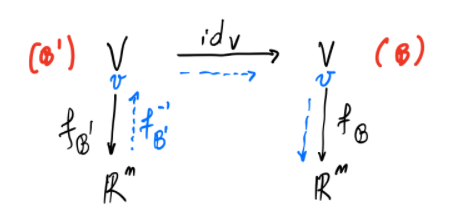
\includegraphics[scale=0.5]{cambiamento_di_base}
\end{center}
\[id_V: V\rightarrow V\]
\[v\mapsto v=id_V(v)\]
($id_V$ è una trasformazione lineare biunivoca) è l'elemento neutro nella composizione delle trasf.lineari da $V$ in se.

\textbf{Richiamo} Se $\mathcal{B}$ è una base, allora l'applicazione
\[f_{\mathcal{B}}: V\rightarrow \mathbb{R}\]
\[v\rightarrow \begin{bmatrix}x_1\\\vdots\\x_n\end{bmatrix}\]
Se $v=x_1v_1+...+x_nv_n$, $\begin{bmatrix}x_1\\\vdots\\x_n\end{bmatrix}=f_{\mathcal{B}}(v)$ è:
\begin{itemize}
  \item Lineare
  \item Biunivoca
\end{itemize}

\begin{center}
  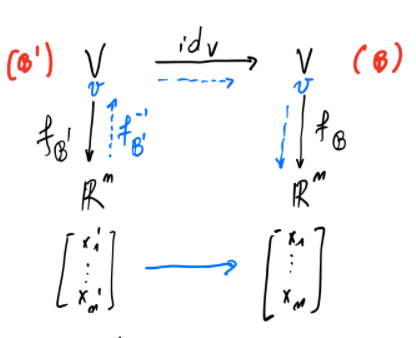
\includegraphics[scale=0.5]{cambiamento_base_2}
\end{center}
\[v=x'_1v'_1+x'_2v'_2+x'_3v'_3=f_{\mathcal{B}'}^{-1}\begin{bmatrix}x_1\\x_2\\x_3\end{bmatrix}\]
\[f_{\mathcal{B}}\circ id_V\circ f_{\mathcal{B}'}^{-1}\]
Siano:

$f_{\mathcal{B}}(v)=\begin{bmatrix}x_1\\\vdots\\x_n\end{bmatrix}$ le coordinate di $v$ in base $\mathcal{B}$

$f_{\mathcal{B}'}(v)=\begin{bmatrix}x'_1\\\vdots\\x'_n\end{bmatrix}$ le coordinate di $v$ in base $\mathcal{B}'$

Allora esiste un'unica applicazione $\Psi$ che rende il diagramma commutativo:
\[\Psi=f_{\mathcal{B}}\circ id_V \circ f_{\mathcal{B}'}^{-1}\]
ed esiste un'unica matrice $B$ tale che:
\begin{itemize}
\item \[f_{\mathcal{B}}=L_B \circ f_{\mathcal{B}'}\]
  \[=L_B\circ f_{\mathcal{B}'}(v) (\in\mathbb{R})\]
  \[L_B(f_{\mathcal{B}'}(v))=B\begin{bmatrix}x_1\\\vdots\\x_n\end{bmatrix}\]
  (con $L_B$ la trasformazione lineare associata alla moltiplicazione per $B$:
  \[L_B: \mathbb{R}^n\rightarrow\mathbb{R}^n\]
  \[Y\mapsto L_B(Y)=BY\]
  \[Y\mapsto Y)\]

\item Se $X=f_{\mathcal{B}}(v)\;\;\;\;\;X'=f_{\mathcal{B}'}(v)$ allora:
  \[X=BX'\]\[\text{ \textbf{Trasformazione delle coordinate}}\]
  Se $\mathcal{B}$ è la base vecchia e $\mathcal{B}'$ è la base nuova, allora le coordinate di un vettor $v$ nella base nuova si esprimono come:
  \[X'=B^{-1}X\]
  \\(\textit{Oss.}: $\Psi(X')=X, \Psi=L_B$ per un'opportuna matrice $B$.)

\item $B$ si chiama la matrice del cambiamento di base e si ottiene come:
  $B_{n\times n}[y_1\dots y_n]$, dove $y_i=\begin{bmatrix}\\ \\ \\\end{bmatrix}$ sono le coordinate di $v_i$ nella base $B$.
  \\Cioè $B=[f_{\mathcal{B}}(v'_1),...,f_{\mathcal{B}}(v'_n)]$, cioè è la matrice che contiene come colonne consecutive le coordinate dei vettori della base nuova espressi nella base vecchia, ovvero:
  \[\mathcal{B}=\mathcal{B}'\cdot B\]

\subsection{Def: Matrice associata a una trasformazione lineare $T$}
(opp. matrice che rappresenta $T$ rispetto alle basi degli spazi vettoriali)
\\L'unica matrice che rende il diagramma commutativo (cioè tale che $f_C\circ T\circ f_{\mathcal{B}}^{-1}=L_A$) si chiama matrice associata a $T$ nelle basi $\mathcal{B}$ e $\mathcal{C}$.
\\In altre parole $f_{\mathcal{C}}\circ T= L_Af_{\mathcal{B}}$, ovvero $f_{\mathcal{C}}(T(v))= Af_{\mathcal{B}}(v)A$.
\\In altre parole:
\[\underline{x}=f_{\mathcal{B}}(v)\]
\[\underline{y}=f_{\mathcal{C}}T((v))\]
\[\Rightarrow \underline{y}=A\underline{x}\]

\subsection{Proposizione}
\begin{itemize}
\item $V$ ha due basi $\mathcal{B}$ e $\mathcal{B}'$, sia $B$ la matrice del cambio di base da $\mathcal{B}$ a $\mathcal{B}'$:
  \[\mathcal{B}'=\mathcal{B}B\]

\item $W$ ha due basi $\mathcal{C}$ e $\mathcal{C}'$, sia $C$ la matrice del cambio di base da $\mathcal{C}$ a $\mathcal{C}'$:
  \[\mathcal{C}'=\mathcal{C}C\]

\item Se $T:V\rightarrow W$ una trasformazione lineare, con
  \begin{itemize}
  \item $A$ è la matrice che rappresenta $T$ nelle basi $\mathcal{B}$ e $\mathcal{C}$.
  \item $A'$ è la matrice che rappresenta $T$ nelle basi $\mathcal{B}'$ e $\mathcal{C}'$.
  \end {itemize}
  
\end{itemize}

\begin{enumerate}

\item Allora $A'=B^{-1}AC$ (cambiamento di matrice che rappresenta $T$)
\item Nel caso in cui $W=V$, e se prendo la stessa base per $V$ (cioe $\mathcal{C}=\mathcal{B}$) e sia $\mathcal{B}'$ un'altra base di $V$.
\\Se $B$ è la matrice del cambiamento di base da $\mathcal{B}$ a $\mathcal{B}'$, la nuova mtrice che rappresenta $T$ nella base $\mathcal{B}'$ è data da:
  \[A'=B^{-1}AB\]
  cioè $A'$ è coniugata tramite la matrice $B$ del cambiamento di base.

\end{enumerate}
\end{itemize}

\subsection{Definizione: matrice simile}
Si dice che una matrice quadrata $A$ è simila ad una matrice $A'\Leftrightarrow\exists\; B$ invertibile tale che:
\[A'=B^{-1}AB\]

\subsection{Proposizione}
Data $T:V\rightarrow V$ (endomorfismo) sia $\mathcal{B}$ una base di $V$ e sia $A$ la matrice (quadrata) associata a $T$ nella base $\mathcal{B}$.
\begin{enumerate}
\item Se $\mathcal{B}'$ è un'altra base di $V$, allora la matrice $A'$ associata a $T$ nella base $\mathcal{B}$ è data da:
  \[A'=D^{-1}AD\]
  Cioè esiste $D$ $n\times n$ invertibile tale che $A'$ è coniugata di $A$ tramite $D$.
  \\Con $D$ invertibile e che rappresenta la matrice del cambiamento di base da $\mathcal{B}$ a $\mathcal{B}'$.

\item Se $A'$ è una matrice simile ad $A$, allora esiste una base $\mathcal{B}'$ di $V$ tale che $A'$ è la matrice che rappresenta $T$ in base $\mathcal{B}'$!

\end{enumerate}

\subsection{Proposizione}
La relazione tra matrici $n\times n$ definita da:
\[A\sim B\Leftrightarrow\exists C\text{ invertibile con } B=C^{-1}AC\]
è una relazione di equivalenza su $\mathcal{M}_n(\mathbb{R})$
\\TODO:DIMOSTRAZIONE R-S-T

\subsection{$\mathcal{M}_n(\mathbb{R})_{/\sim}$ Quoziente modulo la similitudine}
La classe di similitudine di una matrice $A\in \mathcal{M}_n(\mathbb{R})$, denotata con $\mathcal{O}_A$:
\[\mathcal{O}_A:=\{B\in\mathcal{M}_n(\mathbb{R}): A\sim B\}=\{B:\exists C, B=C^{-1}AC\}\]
è l'insieme delle matrici simili ad $A$.

A ogni endomorfismo di $T:V\rightarrow V$ si può associare in modo unico una classe di similitudine (che contiene tutte e sole le matrici che rappresentano $T$ nelle diverse basi).

\subsection{Definizioni: autovettore, autovalore, spettro di $T$, autospazio}
Sia $T:V\rightarrow V$ (endomorfismo) e sia $v\neq\underline{0}_V$:
\begin{itemize}
\item $v$ è un \textbf{autovettore} per $T$ se esiste $\lambda\in\mathbb{R}$ scalare tale che:
  \[T(v)=\lambda v\]
\item Tale $\lambda$ si chiama \textbf{autovalore} relativo all'autovettore $v$ (associato all'autovettore $v$)
\item L'insieme di tutti gli autovalori (se esistono) di una trasformazione $T$ si chiama \textbf{spettro di $T$}
  \[Spec(T)=\{\lambda\in K:\exists v\neq 0, v\in V\text{ con } T(v)=\lambda v\}\]

\item Si chiama \textbf{autospazio} relativo a un autovalore di $\lambda$ di $T$ il sottospazio $V_\lambda \leq V$ definito da:
  \[V_\lambda=\{v\in V:T(v)=\lambda v\}\]

\end{itemize}

\subsection{Osservazione}
Vedremo che lo spettro di $T$ non dipende dalla matrice che rappresenta $T$ in una base, cioè è una nozione intrinseca: se $A,B$ sono due matrici che rappresentanto $T$ in due basi diverse (cioè sono simili), allora $Spec(A)=Spec(B)$ dove $Spec(A)=Spec(L_A)$.
\begin{itemize}
\item $Spec(T)$ (o di una matrice) può essere vuoto.
\item Sia $\lambda_0$ un autovalore di $T$:
  \[V_{\lambda_0}=\{v\in V: T(v)=\lambda_0 V\}\]
  \[=\{v\in V: T(v)-\lambda_0id(v)=0\}\]
  \[=\{v\in V:(T-\lambda_0I)(v)=0\}\]
  \[=Ker(T-\lambda_0I)\neq\{0_V\}\]
\end{itemize}

\subsection{Proposizione}
\begin{enumerate}
\item $\lambda$ è un autovalore per $T\Leftrightarrow T-\lambda id_V$ è una trasformazione singolare (una trasformazione lineare è singolare se ha nucleo non vuoto).
\item Se $v$ è autovettore relativo a $\lambda$, allora non può essere autovettore relativo a un altro scalare $\mu\neq\lambda $, infatti:
  \[Av=\lambda V\text{ e anche } Av=\mu v\]
  \[\Rightarrow \lambda v=\mu v \Leftrightarrow \lambda v-\mu v=0_V\]
  \[(\lambda -\mu)v=0_V\]
  che è una contraddizione perchè $v\neq 0$ perchè autovettore e $\lambda-\mu\neq 0$.

  \item Autovettori relativi ad autovalori distinti sono linearmente indipendenti.

\end{enumerate}

\subsection{Diagonalizzazione di una matrice}
\begin{itemize}
\item Un endomorfismo $T:V\rightarrow V$ di $V$ è diagonalizabile $\Leftrightarrow$ esiste una base di $T$ fatta di autovettori.
  \\$\Rightarrow$ in base $\mathcal{B}$ la matrice che rappresenta $T$ è diagonale.

\item Ogni matrice che rappresenta $T$ in qualche base ha gli stessi autovalori di $T$, cioè:
  \[Spec(L_A)=Spec(A)=Spec(T)\]

\item L'autospazio relativo all'autovalore $lambda $,
  \[V_\lambda=\{v\in V: T(v)=\lambda v\}=Ker(T-\lambda id)\]

\item Autovettori relativi ad autovalori distinti sono indipendenti.

\item $\lambda$ autovalore di $T\Leftrightarrow T-\lambda id_V$ è singolare ($Ker(T-\lambda id_V)\neq\{0_V\}$).

\item Se $A$ è la matrice della trasformazione $L_A:\mathbb{R}^n\rightarrow\mathbb{R}^n$ (nella base canonica) $A$ ha un autovalore $\lambda\Leftrightarrow$ la matrice $(A-\lambda I_n)$ è singolare $\Leftrightarrow$ $Ker(A-\lambda I_n)$ è non banale $\Leftrightarrow det(A-\lambda I_n)=0$.
  
\end{itemize}

\subsection{Polinomio caratteristico}
Si chiama polinomio caratteristico di $T:V\rightarrow V$ il polinomio:
\[p_T(\lambda)=det(T-\lambda id_V)\]

\subsection{Proposizione}
Se $A$ e $B$ sono simili, allora hanno lo stesso polinomio caratteristico: cioè se $A$ e $B$ rappresentano (in basi diverse) la stessa trasformazione $T$: allora
\[det(A-\lambda I_n)=det(B-\lambda I_n)\]
\textbf{Dimostrazione}: $A\sim B\Leftrightarrow \exists C$ invertibile con $B=C^{-1}AC$.
\\Osserviamo che:
\[C^{-1}(A-\lambda I_n)C=\]
\[=(C^{-1}A-C^{-1}\lambda I_n)C\]
\[=C^{-1}AC-C^{-1}\lambda I_nC\]
\[=B-\lambda C^{-1}I_n C\]
\[=B-\lambda I_n\]

Infine:
\[det(B-\lambda I_n)=det(C^{-1}(A-\lambda I_n)C=\]
\[det(C^{-1})det(A-\lambda I_n)det(C)=\]
\[det(C^{-1})det(C)det(A-\lambda I_n)=\]
\[\frac{1}{det(C)}det(C)det(A-\lambda I_n)=\]
\[det(A-\lambda I_n)\]
Quindi possimao dire che $p_T(\lambda)=p_A(\lambda)$ per ogni matrice $A$ nella classe di similitudine.

\subsection{Proprietà del polinomio caratteristico}
\begin{itemize}

\item $p_T(\lambda)=det(A-\lambda I)$ ($A$ che rappresenta $T$ in una base)

\item $p_T(\lambda)$, $(p_A(\lambda))$ è un polinomio:
  \begin{itemize}
  \item di grado $n$ in $\lambda $
  \item Il coefficiente di $\lambda ^n$ è $(-1)^n$
  \item Il coefficiente di $\lambda^{n-1}$ è $(-1)^ntr(A)$ ($traccia(A)=$somma degli el. sulla diagonale)
  \item Il coefficiente di $\lambda ^0=1$ (del termine noto) è $(-1)^0detA=detA$
  \end{itemize}

\item $v\neq 0$ e $Av=\lambda v \Leftrightarrow$
  \[(A-\lambda I)v=0\;\;(v\neq 0)\]
  \[\Leftrightarrow (A-\lambda I)singolare\]
  \[\Leftrightarrow det(A-\lambda I)=0\;\;(p_T(\lambda))\]
  \[\Leftrightarrow\lambda\text{ è radice del polinomio caratteristico}\]

\end{itemize}

\subsection{Corollario}
Se $p_T(\lambda)$ ha $n$ soluzioni distinte, allora $T$ è diagonalizzabile.

\subsection{Def: molteplicità algebrica radice}
Si chiama \textbf{molteplicità algebrica} di una radice $x_0$ (soluzione) di un polinomio $p(x)$ un numero $k$ tale che $(x-x_0)^k|p(x)$ ma $(x-x_0)^{k+1}\nmid p(x)$
  \[p(x)=(x-x_0)^kq(x)\]

\subsection{Def: molteplicità algebrica $\lambda_0$}  
Si chiama \textbf{molteplicità algebrica} di $\lambda_0$ (autovalore di $T$) e si denota con $m_a(\lambda_0)$ la molteplicità algebrica di $\lambda_0$ come radice di $p_T(\lambda)$, cioè:
  \[p_T(\lambda)=(\lambda -\lambda_0)^{m_a(\lambda_0)}(\;\;\;)\]

\subsection{Def: molteplicità geometrica $\lambda_0$}
Si chiama \textit{molteplicità geometrica} di $\lambda_0$ (autovalore di $T$) e si indica con $m_g(\lambda_0)$, la dimensione dell'autospazio di $V_{\lambda_0}$ relativo a $\lambda_0$, cioè la nullità di $T-\lambda_0 I$.
  \\In genere $m_g(\lambda_0)\leq m_a(\lambda_0)$

\subsection{Teorema}
Le seguenti sono equivalenti per $T:V\rightarrow V, \; dim_KV=n$:
\begin{enumerate}
\item $T$ è diagonalizzabile $\Leftrightarrow $

\item $T$ ha tutti i suoi autovalori in $K$ (cioè il polinomio caratteristico si spezza in fattori del tipo $(x-a)^*$ lineari di grado 1) e la molteplicità algebrica di ogni autovalore coincide con la molteplicità geometrica:
  \[m_a(\lambda_0)=m_g(\lambda_0)\;\;\forall\lambda_0\in Spec(T)\]
  quindi se con $Spec(T)=\{\lambda_1,...,\lambda_k\}$ allora $n=m_g(\lambda_1)+...+m_g(\lambda_k)$.

\end{enumerate}

\section{Usi di Gauss-Jordan in vari ambiti}
\subsection{Risolvere $AX=b$}
Si applica GJ alla matrice aumentata $[A|b]\rightarrow[R|b']$ con $A\sim R$ e $[A|b]\sim[R|b']$.

$AX=b$ ha le stesse soluzioni di $RX=b'$. Si risolve a questo punto il sistema ridotto $RX=b'$

\subsection{Rango e base $ImL_A$}
Si applica $A\rightarrow R$.

\textit{Rivedere Corollario $ImL_A$}

Le colonne sono generatori:
\[[A^{(1)},...,A^{(n)}]=A\sim R\]
allora le colonne di $A$ corrispondenti ai pivot sono indipendenti: $A^{(j_1)}...A^{(j_r)}$:
\[rg(A)=dimImL_A=r\]
e $A^{(j_1)}...A^{(j_r)}$ è una base per l'immagine.

\subsection{Trovare $Ker(L_A)=KerA$}
\[KerT=\{v\in V:T(v)=0\}\]
\[KerL_A=\{X\in\mathbb{R}^n:L_A(X)=\underline{0}\}=\]
\[\{X\in\mathbb{R}^n:AX=\underline{0}\}=\]
\[=\text{spazio delle soluzioni del sistema lineare omogeneo associato ad } A\]
$KerA=$Soluzioni di $AX=0$: applicando GJ ad $A$: $A\sim R$ e risolvo ora $RX=0$.

\subsection{Estrazione insieme di vettori indipendenti}
Per il problema di estrarre un insieme indipendente più grande possibile da un insieme di vettori di $\mathbb{R}^n$: ci si chiede dato $\{v_1,...v_k\}\subseteq\mathbb{R}^n$, qual è una base per $Span(v_1,...,v_n)$ da estrarre da $\{v_1,...v_k\}$.
\\Costruisco la matrice $A=\begin{bmatrix}v_1&\dots&v_k\end{bmatrix}_{nxk}$:
\\$A\sim^{GJ}R$: le colonne di $A$ corrispondenti alle colonne di $R$ dove si trovano i pivot sono indipendenti.

\subsection{Completamento a un base di $\mathbb{R}$}
Dati $v_1,...,v_k\in\mathbb{R}^n$ indipendenti, voglio completare $\{v_1,...,v_k\}$ a una base di $\mathbb{R}^n$ (se $k<n$).

In questo caso formo un insieme $\{v_1,...,v_k,e_1,...,e_n\}$. Costruisco 
\[A=\begin{bmatrix}v_1 & \dots & v_k & e_1 & \dots & e_n\end{bmatrix}\]
Applico GJ: $A\sim R$ e scelgo le colonne di $A$ corrispondenti ai pivot.

\subsection{Trovare base di $U+W\text{ e } U\cap W$}
Per trovare una base di $U+W\text{ e } U\cap W$ date una base di $U$ e una di $W$.



\end{document}
